\section{Nội dung}
%1111111111111111111111111111111111111111111111111111111111111
\subsection{Tích hợp dữ liệu - Integration}
\subsubsection{Định nghĩa sự tích hợp dữ liệu}
Tích hợp dữ liệu là kết hợp dữ liệu từ nhiều nguồn vào một nơi lưu trữ thống nhất để tiện cho những thao tác về sau. Dữ liệu ở đây có thể bao gồm nhiều cơ sở dữ liệu, khối dữ liệu, hoặc các file dữ liệu.

\subsubsection{Kiểm tra nhận diện thực thể}
Có vấn đề về nhận diện thực thể (\textit{entity identification}) trong 2 dataset này. Cụ thể, ở file \code{heart-c.arff}, thuộc tính thứ 3 tên là \code{cp}, còn ở file \code{heart-h.arff}, thuộc tính thứ 3 tên là \code{chest\_pain}.

Hướng giải quyết: Đổi tên thuộc tính \code{chest\_pain} ở file \code{heart-h.arff} thành \code{cp}.
\begin{figure}[H]
\centering
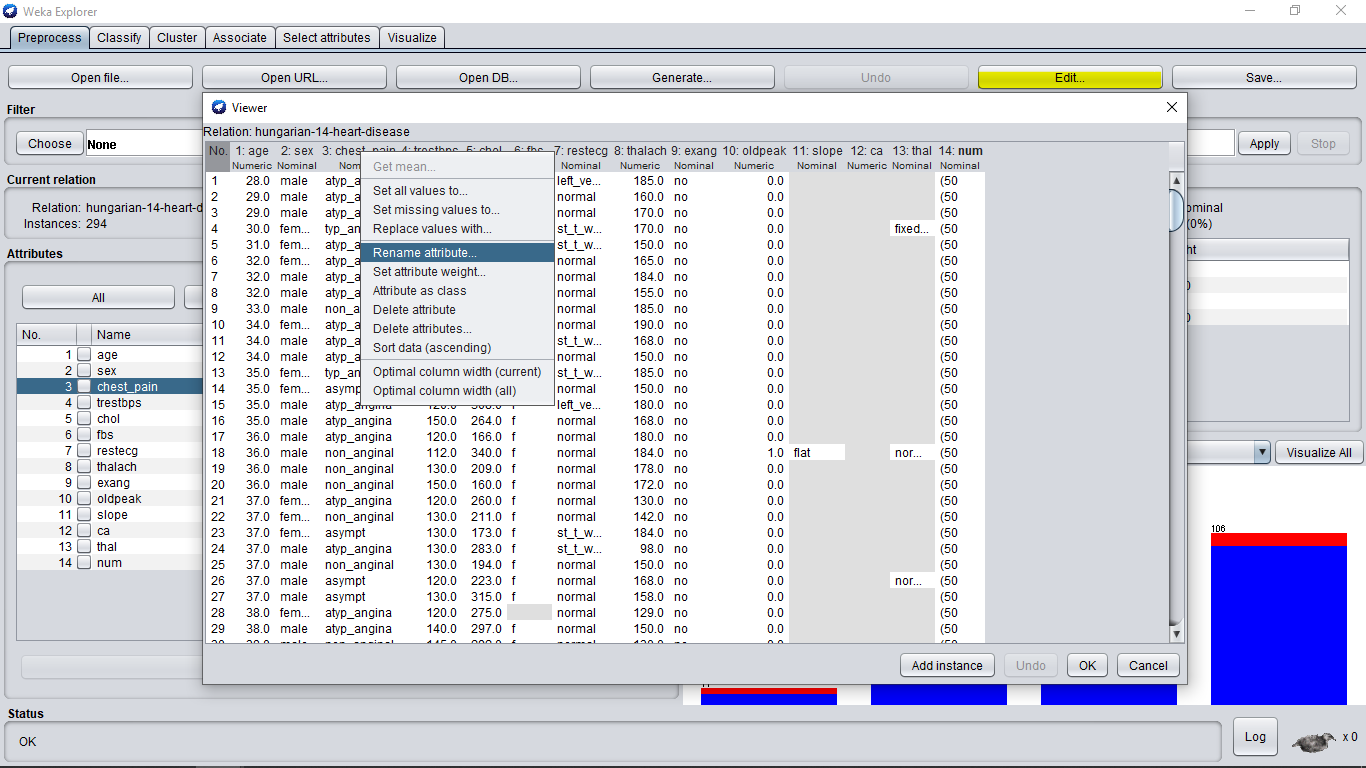
\includegraphics[width=0.98\textwidth]{1/b1.png}
\caption{Ở tab \textit{Preprocessing}, chọn \textit{Edit}, chuột phải phải vào thuộc tính \code{cp} và chọn \textit{Rename attribute...}}
\end{figure}

\begin{figure}[H]
\centering
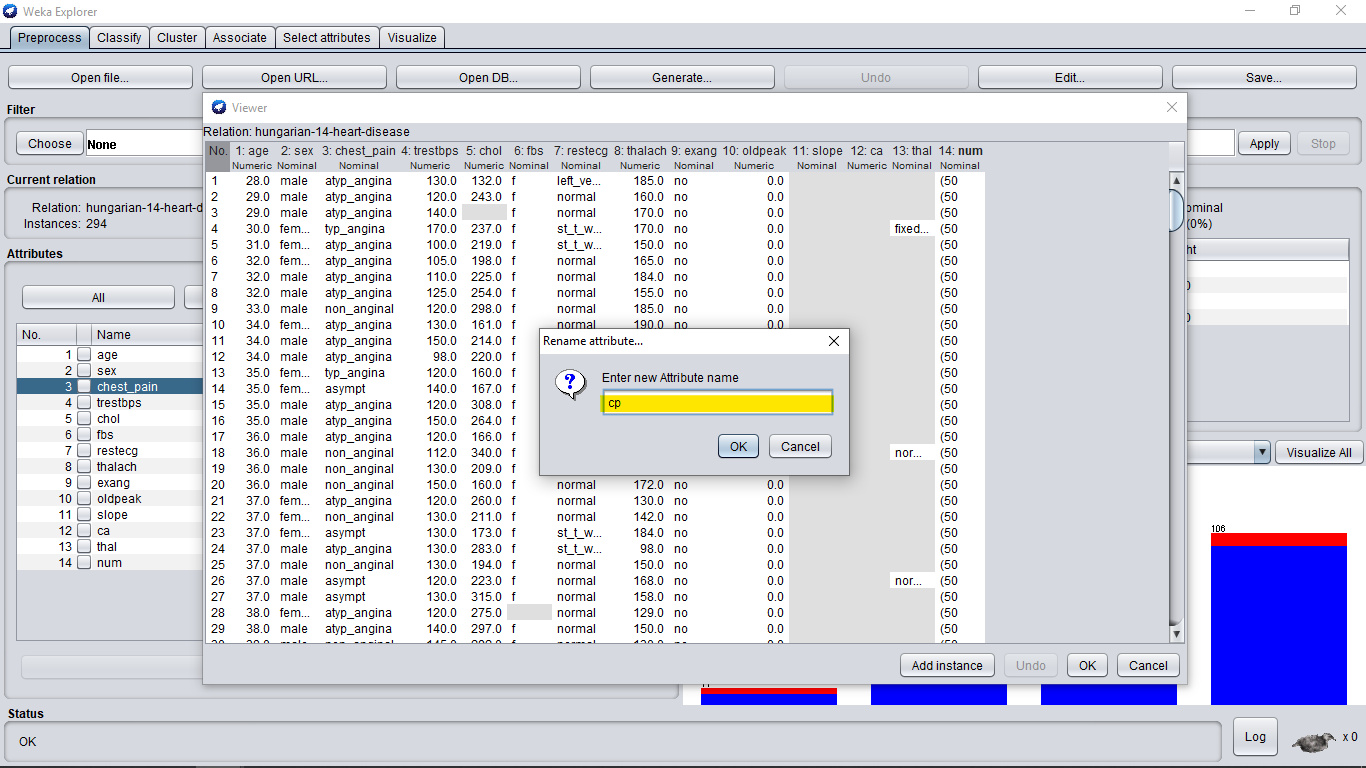
\includegraphics[width=0.98\textwidth]{1/b2.png}
\caption{Điền tên cần đổi vào cửa sổ hiện lên và nháy \textit{OK}.}
\end{figure}

\subsubsection{Kiểm tra dữ liệu dư thừa}
Ta dùng \textit{Karl Pearson} để kiểm tra sự tương quan giữa các thuộc tính số và \textit{Chi-Square} để kiểm tra sự tương quan giữa các thuộc tính rời rạc.
% Please add the following required packages to your document preamble:
% \usepackage{booktabs}
% Please add the following required packages to your document preamble:
% \usepackage{booktabs}
\begin{table}[H]
\centering
\renewcommand{\arraystretch}{1.5}
\caption {\textit{Correlation} giữa các thuộc tính số của file \code{heart-c.arff}.}
\begin{tabular}{@{}lccccc@{}}
\toprule
                  & \textbf{age} & \textbf{trestbps} & \textbf{chol} & \textbf{thalach} & \textbf{oldpeak} \\ \midrule
\textbf{trestbps} & 0.279        &                   &               &                  &                  \\
\textbf{chol}     & 0.214        & 0.123             &               &                  &                  \\
\textbf{thalach}  & -0.399       & -0.047            & 0.010         &                  &                  \\
\textbf{oldpeak}  & 0.210        & 0.193             & 0.054         & -0.344           &                  \\
\textbf{ca}       & 0.365        & 0.103             & 0.122         & -0.263           & 0.294            \\ \bottomrule
\end{tabular}
\end{table}

% Please add the following required packages to your document preamble:

\begin{table}[H]
\centering
\renewcommand{\arraystretch}{1.5}
\caption {\textit{Chi-Square} giữa các thuộc tính rời rạc của file \code{heart-c.arff} (những giá trị gạch chân thể hiện hai thuộc tính có sự tương quan).}
\begin{tabular}{@{}llllllll@{}}
\toprule
                     & \textbf{sex} & \textbf{cp} & \textbf{fbs} & \textbf{restecg} & \textbf{exang} & \textbf{slope} & \textbf{thal} \\ \midrule
\textbf{cp} & 6.822        &                      &              &                  &                &                &               \\
\textbf{fbs}         & 0.614        & 3.886                &              &                  &                &                &               \\
\textbf{restecg}     & 3.697        & 9.688                & 2.297        &                  &                &                &               \\
\textbf{exang}       & 6.081        & {\ul 67.348}         & 0.2          & 2.976            &                &                &               \\
\textbf{slope}       & 0.648        & {\ul 27.747}         & 3.373        & 10.947           & {\ul 25.131}   &                &               \\
\textbf{thal}        & {\ul 44.626} & {\ul 41.892}         & 5.542        & 3.526            & {\ul 32.959}   & {\ul 35.283}   &               \\
\textbf{num}         & {\ul 23.914} & {\ul 81.686}         & 0.238        & 10.023           & {\ul 57.799}   & {\ul 47.507}   & {\ul 85.304}  \\ \bottomrule
\end{tabular}
\end{table}

\begin{table}[H]
\centering
\renewcommand{\arraystretch}{1.5}
\caption {\textit{Correlation} giữa các thuộc tính số của file \code{heart-h.arff}.}
\begin{tabular}{@{}lllll@{}}
\toprule
                  & \textbf{age} & \textbf{trestbps} & \textbf{chol} & \textbf{thalach} \\ \midrule
\textbf{trestbps} & 0.245        &                   &               &                  \\
\textbf{chol}     & 0.091        & 0.084             &               &                  \\
\textbf{thalach}  & -0.459       & -0.185            & -0.128        &                  \\
\textbf{oldpeak}  & 0.178        & 0.207             & 0.109         & -0.303           \\ \bottomrule
\end{tabular}
\end{table}

\begin{table}[H]
\centering
\renewcommand{\arraystretch}{1.5}
\caption {\textit{Chi-Square} giữa các thuộc tính rời rạc của file \code{heart-h.arff} (những giá trị gạch chân thể hiện hai thuộc tính có sự tương quan).}
\begin{tabular}{@{}llllllll@{}}
\toprule
                 & \textbf{sex} & \textbf{cp}  & \textbf{fbs} & \textbf{restecg} & \textbf{exang} & \textbf{slope} & \textbf{thal} \\ \midrule
\textbf{cp}      & {\ul 19.042} &              &              &                  &                &                &               \\
\textbf{fbs}     & 2.593        & 1.290        &              &                  &                &                &               \\
\textbf{restecg} & 7.379        & {\ul 29.535} & 1.580        &                  &                &                &               \\
\textbf{exang}   & 9.632        & {\ul 82.540} & 4.088        & 7.728            &                &                &               \\
\textbf{slope}   & 5.012        & {\ul 66.018} & 15.987       & 11.918           & {\ul 176.898}  &                &               \\
\textbf{thal}    & 0.657        & 9.042        & 4.921        & 1.927            & 3.277          & 2.252          &               \\
\textbf{num}     & {\ul 21.876} & {\ul 95.811} & 8.084        & 2.758            & {\ul 100.591}  & {\ul 110.521}  & 10.201        \\ \bottomrule
\end{tabular}
\end{table}

\textit{Ta thấy các thuộc tính có mức độ tương quan không quá cao nên không thể loại bỏ thuộc tính nào. Vậy, không có vấn đề dư thừa dữ liệu trong hai dataset này.}

\subsubsection{Kiểm tra mâu thuẫn dữ liệu}
Kiểm tra từng thuộc tính của 2 dataset, ta thấy không có sự mâu thuẫn dữ liệu (data value conflicts) trong 2 dataset này.

\subsubsection{Tích hợp dữ liệu}
Sau khi tích hợp, dataset mới có 597 mẫu và 14 thuộc tính.
\begin{figure}[H]
\centering
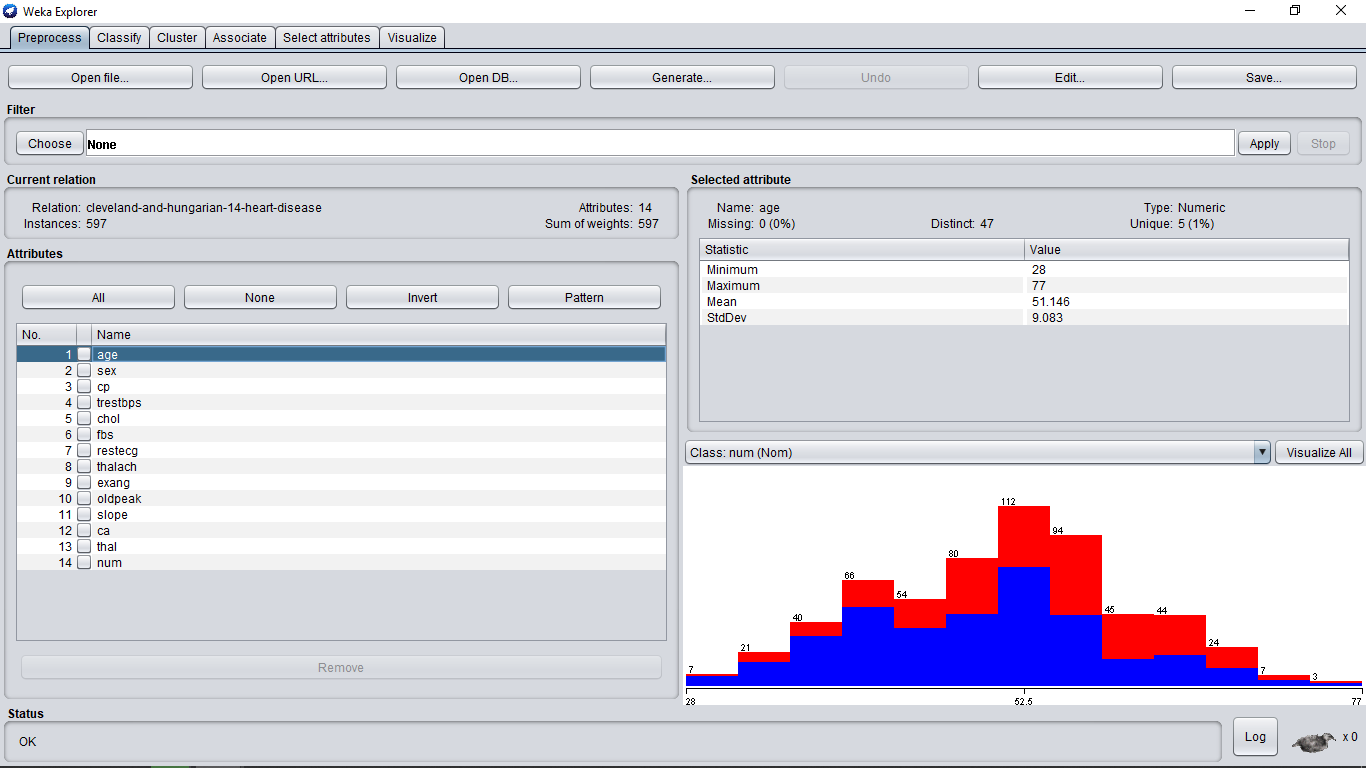
\includegraphics[width=0.98\textwidth]{1/f.png}
\caption{Dataset sau khi tích hợp.}
\end{figure}


%2222222222222222222222222222222222222222222222222222222
\subsection{Tóm tắt mô tả dữ liệu – Descriptive data summarization }
\subsubsection{Xét thuộc tính age}
\begin{itemize}
	\item[--]Trung bình: mean = 51.146.
	\item[--]Độ lệch chuẩn: sd = 9.038.
	\item[--]Giá trị lớn nhất: maximum = 77.
	\item[--]Giá trị nhỏ nhất: minimum = 28.
\end{itemize}
\begin{figure}[H]
\centering
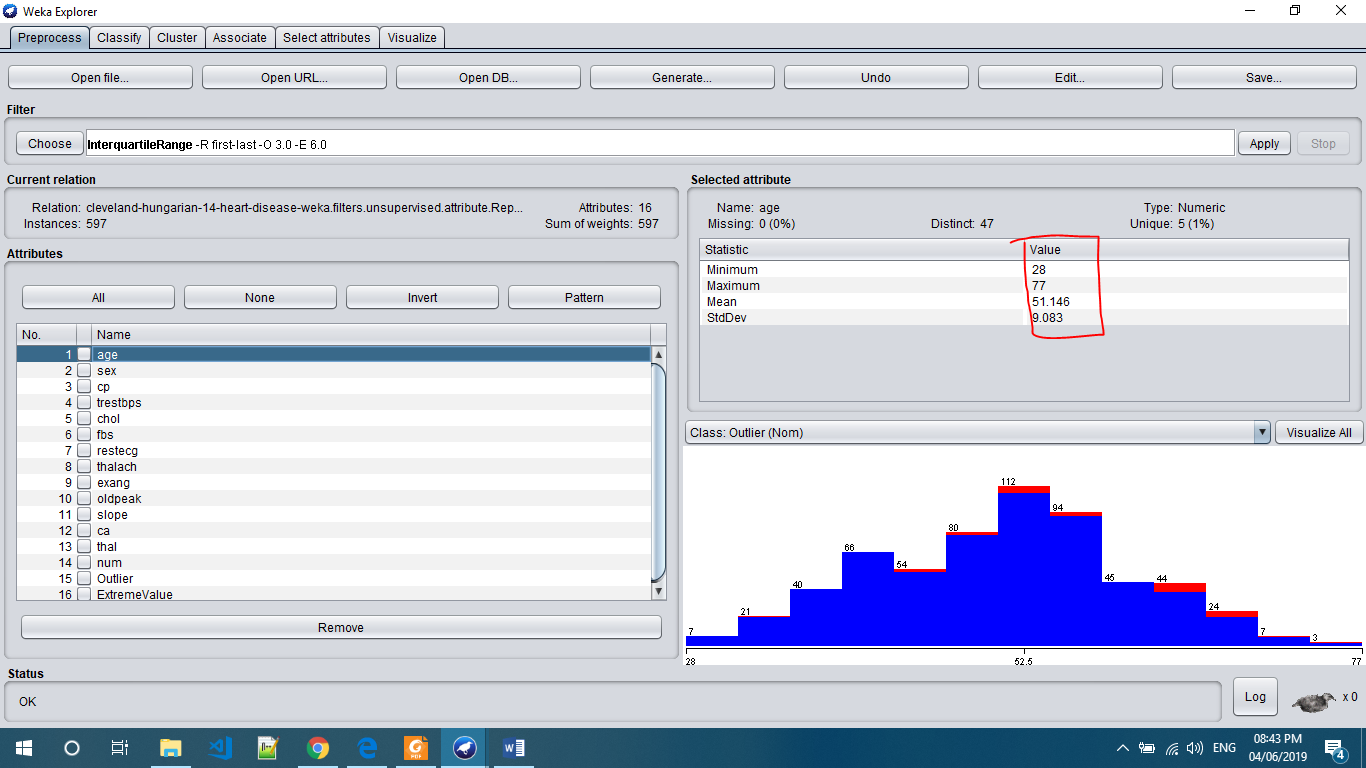
\includegraphics[width=0.98\textwidth]{2/1.png}
\caption{Thuộc tính age.}
\end{figure}

\subsubsection{Five-number summary của thuộc tính age}
\begin{itemize}
	\item[--]Minimum = 28.
	\item[--]Q1 = 44.
	\item[--]Median = 52.
	\item[--]Q3 = 58.
	\item[--]Maximum = 77.
\end{itemize}
\begin{figure}[H]
\centering
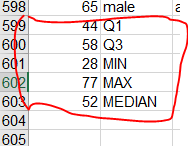
\includegraphics[width=0.4\textwidth]{2/2.png}
\caption{Weka chỉ cung cấp minimum và maximum. Q1, Q3 và median được nhóm chuyển file arff sang csv sao đó sử dụng excel để tìm các giá trị Q1, Q3 và median.}
\end{figure}

\subsubsection{Thông tin thuộc tính}
\begin{itemize}
	\item[--]Thuộc tính số (numeric):  age, trestbps, chol, thalach, oldspeak, ca (6 thuộc tính). 
	\item[--]Thuộc tính có thứ tự (ordernal): restecg, slope, thal, num (4 thuộc tính).
	\item[--]Thuộc tính rời rạc/danh sách (categorical/nominal): sex, cp, fbs, exang (4 thuộc tính).
\end{itemize}

\subsubsection{Ý nghĩa của đồ thị trong cửa sổ Explorer}
\begin{figure}[H]
\centering
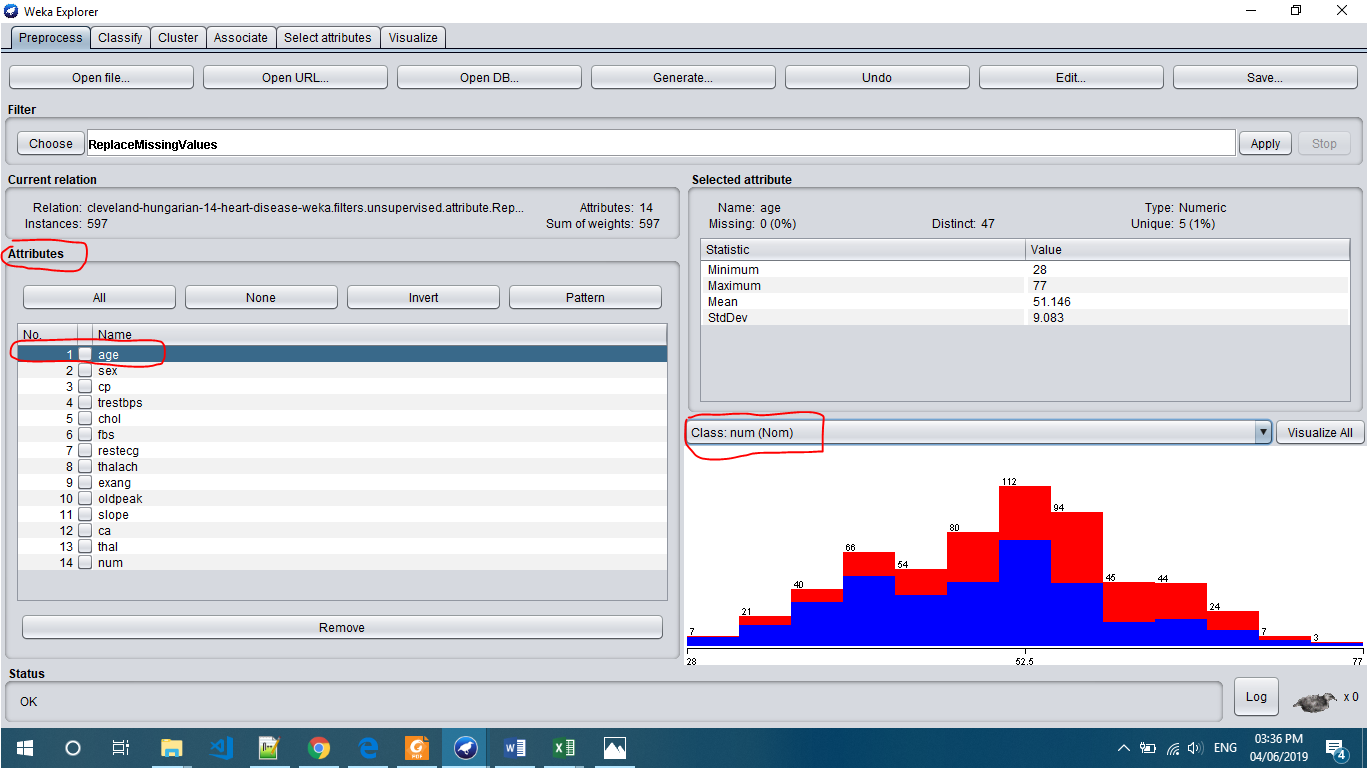
\includegraphics[width=0.98\textwidth]{2/3.png}
\caption{Tên đồ thị: Đồ thị phân bố của thuộc tính.}
\end{figure}

\begin{itemize}
	\item[--]Đồ thị này là đồ thị để thể hiện sự phân bố của thuộc tính hiện được chọn (nền xanh) ở khung Attributes và được phân lớp (classification) theo thuộc tính được chọn ở box Class.
	\item[--]Tên đồ thị: Đồ thị phân bố của thuộc tính. 
	\item[--]Màu xanh ứng với num có label <50 (không mắc bệnh). Màu đỏ ứng với num có label >50\_1 (măc bệnh mức 1).(do mức 2, 3, 4 không có nên trên đồ thị không hiển thị).
	\item[--]Mỗi cột biểu diễn một khoảng tuổi (đang xét theo thuộc tính tuổi), giá trị trên mỗi cột là số lượng instances có ‘age’ thuộc khoảng đó.
	\item[--]Đồ thị biểu diễn phân bố tuổi và tỉ lệ giữa người có bệnh và không có bệnh trên mỗi khoảng tuổi được chia. Ví dụ, ở khoảng [28, 31.769] có 7 người tỉ lệ người không mắc bệnh trong độ tuổi này chiếm cao hơn tỉ lệ người mắc bệnh mức 1 (màu xanh chiếm gần hết cột).
\end{itemize}

\subsubsection{Đồ thị phân bố của các thuộc tính còn lại}
\begin{figure}[H]
    \centering % <-- added
   \begin{subfigure}{0.38\textwidth}
  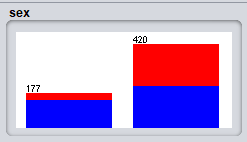
\includegraphics[width=\linewidth]{2/4.png}
  \caption{sex}
  \label{fig:1}
\end{subfigure}\hfil % <-- added
\begin{subfigure}{0.38\textwidth}
  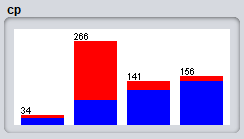
\includegraphics[width=\linewidth]{2/5.png}
  \caption{chest\_pain}
  \label{fig:3}
\end{subfigure}

\medskip
\begin{subfigure}{0.38\textwidth}
  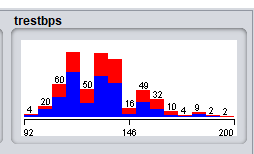
\includegraphics[width=\linewidth]{2/6.png}
  \caption{trestbps}
  \label{fig:1}
\end{subfigure}\hfil % <-- added
\begin{subfigure}{0.38\textwidth}
  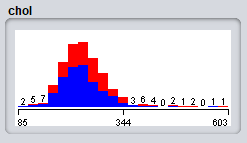
\includegraphics[width=\linewidth]{2/7.png}
  \caption{chol}
  \label{fig:3}
\end{subfigure}

\medskip
\begin{subfigure}{0.38\textwidth}
  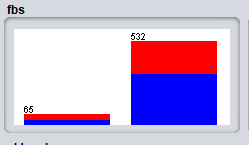
\includegraphics[width=\linewidth]{2/8.png}
  \caption{fbs}
  \label{fig:4}
\end{subfigure}\hfil % <-- added
\begin{subfigure}{0.38\textwidth}
  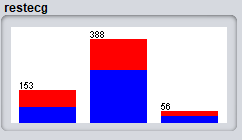
\includegraphics[width=\linewidth]{2/9.png}
  \caption{restecg}
  \label{fig:6}
\end{subfigure}

\medskip
\begin{subfigure}{0.38\textwidth}
  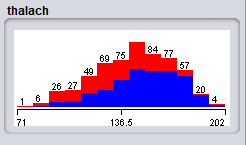
\includegraphics[width=\linewidth]{2/10.png}
  \caption{thalach}
  \label{fig:4}
\end{subfigure}\hfil % <-- added
\begin{subfigure}{0.38\textwidth}
  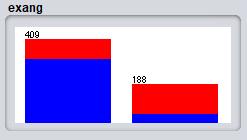
\includegraphics[width=\linewidth]{2/11.png}
  \caption{exang}
  \label{fig:6}
\end{subfigure}

\medskip
\begin{subfigure}{0.38\textwidth}
  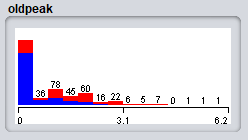
\includegraphics[width=\linewidth]{2/12.png}
  \caption{oldspeak}
  \label{fig:4}
\end{subfigure}\hfil % <-- added
\begin{subfigure}{0.38\textwidth}
  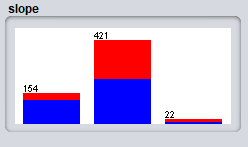
\includegraphics[width=\linewidth]{2/13.png}
  \caption{slop}
  \label{fig:6}
\end{subfigure}

\caption{Đồ thị phân bố của các thuộc tính còn lại (1).}
\label{fig:images}
\end{figure}

\begin{figure}[H]
    \centering % <-- added
   \begin{subfigure}{0.38\textwidth}
  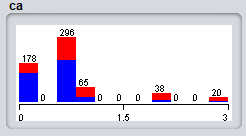
\includegraphics[width=\linewidth]{2/14.png}
  \caption{ca}
  \label{fig:1}
\end{subfigure}\hfil % <-- added
\begin{subfigure}{0.38\textwidth}
  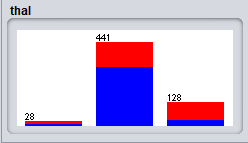
\includegraphics[width=\linewidth]{2/15.png}
  \caption{thal}
  \label{fig:3}
\end{subfigure}

\medskip
\begin{subfigure}{0.38\textwidth}
  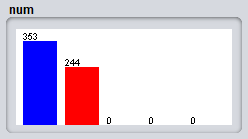
\includegraphics[width=\linewidth]{2/16.png}
  \caption{num}
  \label{fig:1}
\end{subfigure}\hfil % <-- added
\caption{Đồ thị phân bố của các thuộc tính còn lại (2).}
\label{fig:images}
\end{figure}

\subsubsection{Nhận xét}
Đồ thị thể hiện trực quan mối liên hệ giữa 2 thuộc tính bất kỳ trong tập dữu liệu (ví dụ đang xét là giữa thuộc tính \textit{num} với các thuộc tính còn lại). Từ đồ thị có thể nhận thấy được một số thuộc tính có khả năng dùng để phân loại xem có mắc bệnh hay không (sẽ được thể hiện cụ thể hơn ở phần Visualize mà Weka hỗ trợ nhưng có thể phần nào trực quan xem được).

Đồ thị đối với dữ liệu rời rạc (nominal/categorize) thì các cột rời nhau, còn đồ thị có giá trị liên tục thì các cột kề nhau, mỗi cột là một khoảng (mỗi khoảng chứa một số lượng instance có giá trị thuộc khoảng đó).

Các giá trị của thuộc tính (min, max, mean) đối với dữ liệu số sẽ được thể hiện trực quan trên đồ thị.

\subsubsection{Đồ thị "scatter"}
Thuật ngữ sử dụng trong textbook để đặt tên cho đồ thị ở mục Visualize là “scatter plot”. 
\begin{itemize}
	\item[--]Theo nhóm, các thuộc tính có vẽ dẫn đến bệnh tim là: oldspeak (không mắc bệnh trong khoản 0 – 1.6, lớn hơn 1.6 khả năng mắc bệnh cao), exang (no – khả năng không mắc bệnh cao, yes – khả năng mắc bệnh cao), thalach (<136.5 – khả năng mắc bệnh cao, >136.5 – thường không mắc bệnh), slope (up – không mắc bệnh cao, flat – khả năng mắc bệnh cao).
	\item[--]Khả năng dự đoán bệnh tim tốt nhất là thuộc tính exang.
\end{itemize}
\begin{figure}[H]
\centering
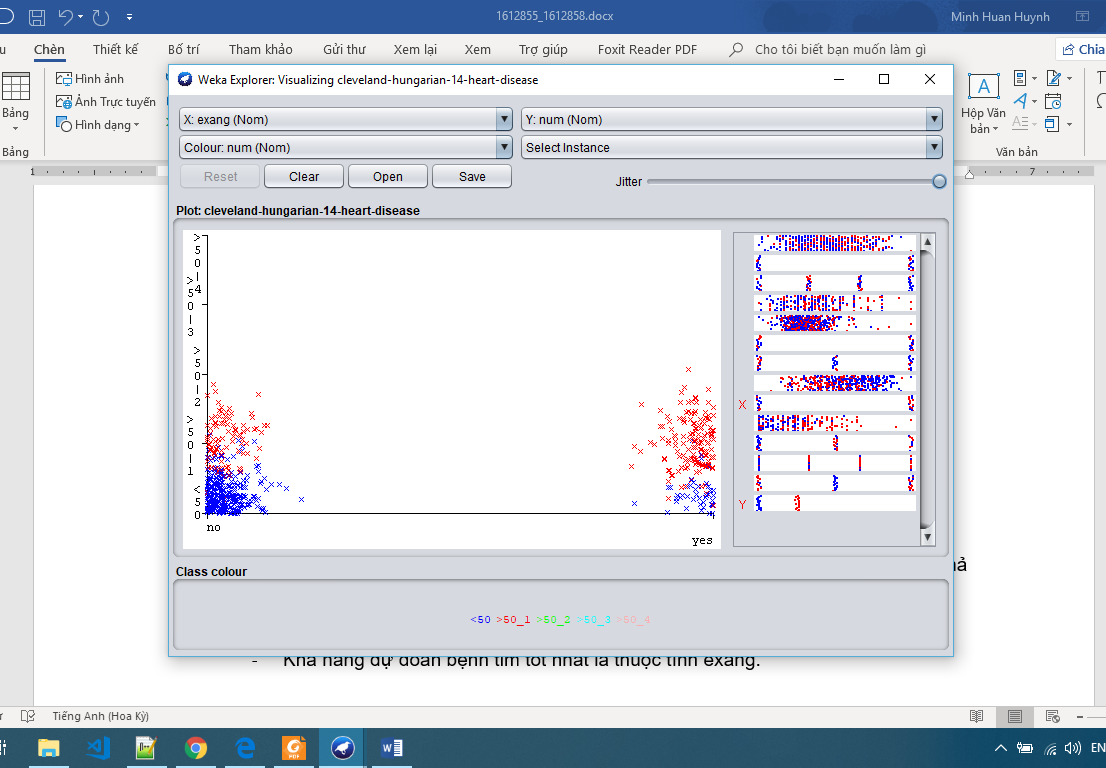
\includegraphics[width=0.98\textwidth]{2/17.png}
\caption{Thuộc tính exang dự đoán tốt nhất.}
\end{figure}

\subsubsection{Những cặp thuộc tính có vẻ tương quan với nhau}
Dựa vào quan sát đồ thị "scatter", ngoài những cặp thuộc tính giữa num và các thuộc tính khác như trên, thì những cặp sau đây có vẻ tương quan với nhau: (slop, cp), (slop, exang), (exang, cp).


%333333333333333333333333333333333333333333333333333333333333333333333
\subsection{Chọn lọc dữ liệu - Selection}
\begin{itemize}
	\item Có 14 thuộc tính trong datasets trước khi xử lý dữ liệu.
	\begin{figure}[H]
\centering
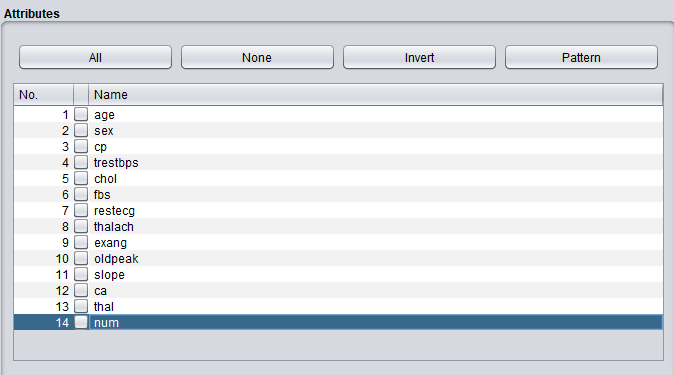
\includegraphics[width=0.98\textwidth]{3/1.png}
\caption{Có 14 thuộc tính trước khi xử lý dữ liệu.}
\end{figure}
\item Các lựa chọn khác nhau để lựa chọn thuộc tính là:
\begin{itemize}
	\item Các phương pháp đánh giá:
	\begin{itemize}
		\item CfsSubsetEval: Đánh giá giá trị của một tập hợp con các thuộc tính bằng cách xem xét khả năng dự đoán riêng của từng tính năng cùng với mức độ dư thừa giữa chúng.
		\item ClassifierSubsetEval: Đánh giá các tập hợp thuộc tính trên dữ liệu huấn luyện hoặc một bộ kiểm tra riêng biệt.
		\item CorrelationAttributeEval: Đánh giá giá trị của một thuộc tính bằng cách đo lường mối tương quan (Pearson's) giữa nó và lớp. Các thuộc tính danh nghĩa được xem xét trên một giá trị theo cơ sở giá trị bằng cách coi mỗi giá trị là một chỉ báo.
		\item GainRatioAttributeEval: Đánh giá theo độ đo tỉ lệ đạt được với các lớp. với công thức tính gain là GainR(Class, Attribute) = (H(Class) - H(Class | Attribute)) / H(Attribute).
		\item OneRAttributeEval: Đánh giá giá trị của một thuộc tính bằng cách sử dụng trình phân loại OneR.
		\item PrincipalComponents: Thực hiện phân tích thành phần chính (chọn ra các thành phần chính) nhằm biến đổi dữ liệu (transformation data).
		\item ReliefFAttributeEval: Đánh giá giá trị của một thuộc tính bằng cách lặp lại việc lấy mẫu (sampling) của một instance và xem xét giá trị của thuộc tính đã cho với instance gần nhất của cùng một lớp và khác lớp.
		\item SymmetricalUncertAttributeEval: Đánh giá giá trị của một thuộc tính bằng cách đo độ không đảm bảo đối xứng đối với lớp.
		\item WrapperSubsetEval: đánh giá bằng tập bao các phân loại (“wrapper” method wraps a classifier in cross-validation loop.
		
	\end{itemize}
	\item Các phương pháp tìm kiếm (chọn thuộc tính theo nhu cầu):
	\begin{itemize}
	\item BestFirst: Tìm kiếm tập con không gian các thuộc tính bằng tham lam tăng cường với cơ sở quay lui. 
	\item GreedyStepwise: Phương pháp tìm kiếm tham lam tiến hay lùi thông qua tập con không gian các thuộc tính.
	\item Ranker: xếp hạng các thuộc tính theo giá trị nó được đánh giá.
	\end{itemize}
	
	
\end{itemize}
\item So sánh các phương pháp giữa weka và textbook: trong textbook không thấy phương pháp tìm kiếm (chọn thuộc tính theo yêu cầu) là BestFirst và Ranker.
\end{itemize}

%44444444444444444444444444444444444444444444444444444444444
\subsection{Làm sạch dữ liệu - Cleaning}
\subsubsection{Missing values (dữ liệu thiếu)}
\begin{itemize}
	\item Các phương pháp xử lý dữ liệu thiếu: 
	\begin{itemize}
		\item	Bỏ qua bộ đó (ignore the tuple).
\item	Điền các dữ liệu thiếu bằng phương pháp thủ công (mannually).
\item	Sử dụng giá trị hằng ngoại vi (global constant) để điền: “Unknown” hay “$\infty$”.
\item	Dùng thuộc tính trung bình (mean) để điền các giá trị thiếu.
\item	Sử dụng thuộc tính trung bình cho tất cả các mẫu thuộc cùng một lớp với bộ dữ liệu đã cho.
\item	Dùng giá trị có thể xảy ra nhất để điền vào giá trị còn thiếu.

	\end{itemize}
	\item Weka đã cài đặt phương pháp: thay thế dữ liệu bằng giá trị trung bình hay mode, thay thế giá trị thiếu bằng hằng số do người dùng đặt, thay thế giá trị thiếu bằng giá trị có thể xảy ra nhất.
	\item Chọn phương pháp điền giá trị thiếu bằng mean hay mode. Vì:
	\begin{itemize}
	\item	không thể tiến hành điền mannual vì dữ liệu thiếu nhiều ở thuộc tính ca (50\%), thal (45\%), slope (32\%) và không thể biết được nên điền như thế nào.
\item	Nếu chọn lược bỏ các tuple thiếu thì lại làm mất tính khách quan dữ liệu.
\item	Chỉ có 1 số thuộc tính bị thiếu nên nhóm nghĩ tốt nhất là chọn ReplaceMissingValue by mean or mode sẽ đảm bảo. 

	\end{itemize}
\end{itemize}

\subsubsection{Noisy data (dữ liệu nhiễu)}
\begin{itemize}
\item Các phương pháp loại bỏ dữ liệu nhiễu:
\begin{itemize}
\item	Phương pháp phân khoảng hay chia giỏ (bining): Chia giỏ theo giá trị trung bình (bin mean), chia giỏ theo trung vị (bin median), chia giỏ theo biên (bin boundaries).
\item	Hồi quy (regression)
\item	Phân cụm, gom nhóm (clustering)

\end{itemize}
\item Weka hỗ trợ: Hồi quy 

\end{itemize}

\subsubsection{Outlier data (dữ liệu ngoại lệ/ dữ liệu tạp)}
\begin{itemize}
\item Các phương pháp:
\begin{itemize}
\item	Gom cụm (Clustering)
\item	Numeric outlier (IQR): điểm dữ liệu tạp nằm ngoài khoảng interquartile (IQR).
\item	Z-score

\end{itemize}
\item Dò tìm dữ liệu tạp bằng Weka:
\begin{figure}[H]
\centering
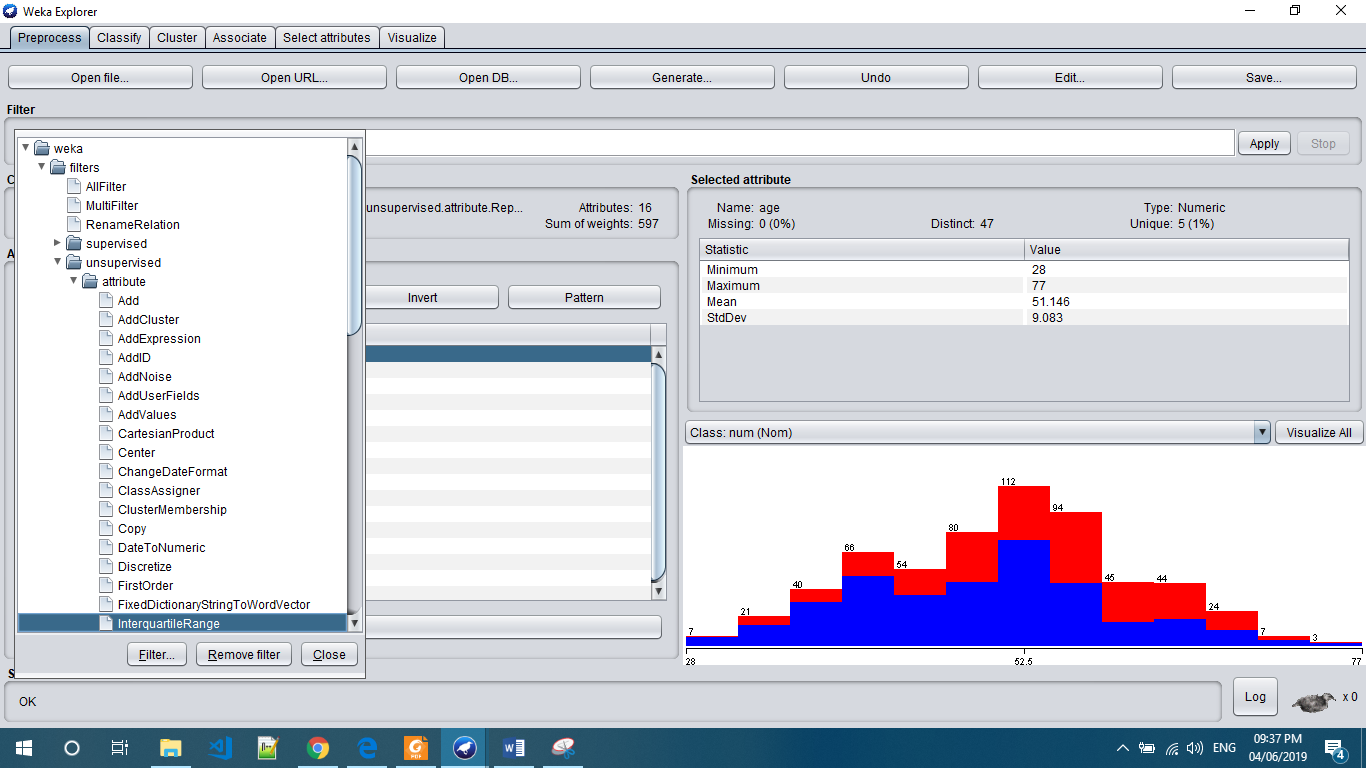
\includegraphics[width=0.98\textwidth]{4/1.png}
\caption{B1 - Mục $Filter \rightarrow Choose \rightarrow filters \rightarrow unsupervised \rightarrow attribute \rightarrow InterquartileRange$.}
\end{figure}

\begin{figure}[H]
\centering
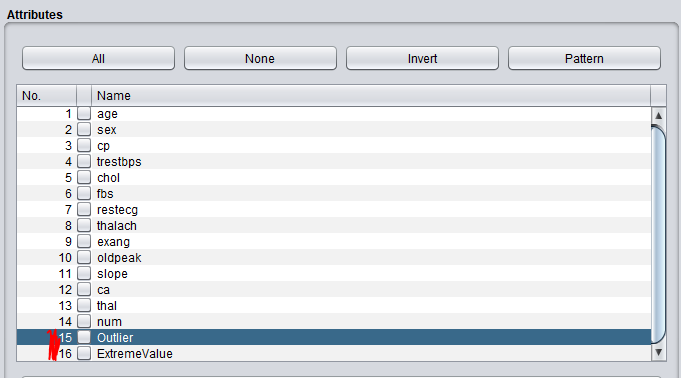
\includegraphics[width=0.98\textwidth]{4/2.png}
\caption{B2 - Nhấn apply, sẽ xuất hiện thêm 2 thuộc tính trong mục Attributes là Outlier và ExtremeValue.}
\end{figure}

\begin{figure}[H]
\centering
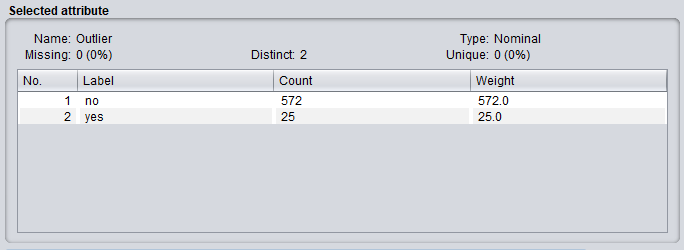
\includegraphics[width=0.98\textwidth]{4/3.png}
\caption{B3 - Chọn thuộc tính Outlier để xem kết quả, có dữ liệu tạp hay không.}
\end{figure}
\item Có dữ liệu tạp trong dataset (như hình trên) là 25 (thuộc tính gần cuối là thuộc tính outlier, file được lưu lại sau khi thực hiện các bước trên).

\begin{figure}[H]
\centering
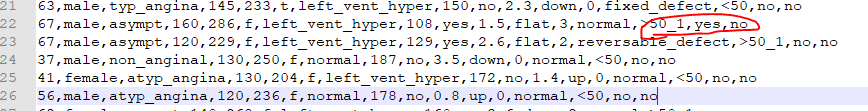
\includegraphics[width=0.98\textwidth]{4/4.png}
%\caption{B3: Chọn thuộc tính Outlier để xem kết quả, có dữ liệu tạp hay không.}
\end{figure}
\begin{figure}[H]
\centering
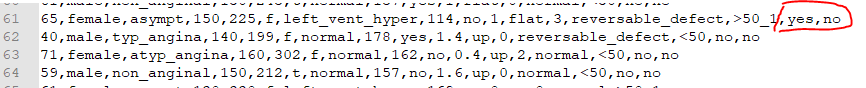
\includegraphics[width=0.98\textwidth]{4/5.png}
%\caption{B3: Chọn thuộc tính Outlier để xem kết quả, có dữ liệu tạp hay không.}
\end{figure}
\begin{figure}[H]
\centering
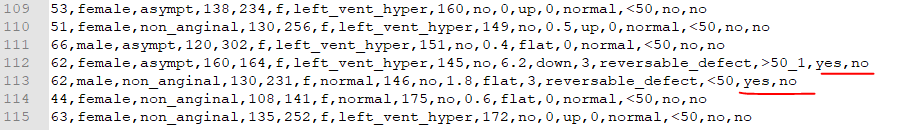
\includegraphics[width=0.98\textwidth]{4/6.png}
%\caption{B3: Chọn thuộc tính Outlier để xem kết quả, có dữ liệu tạp hay không.}
\end{figure}
\item Lưu \code{heart-cleaned.arff}.
\begin{figure}[H]
\centering
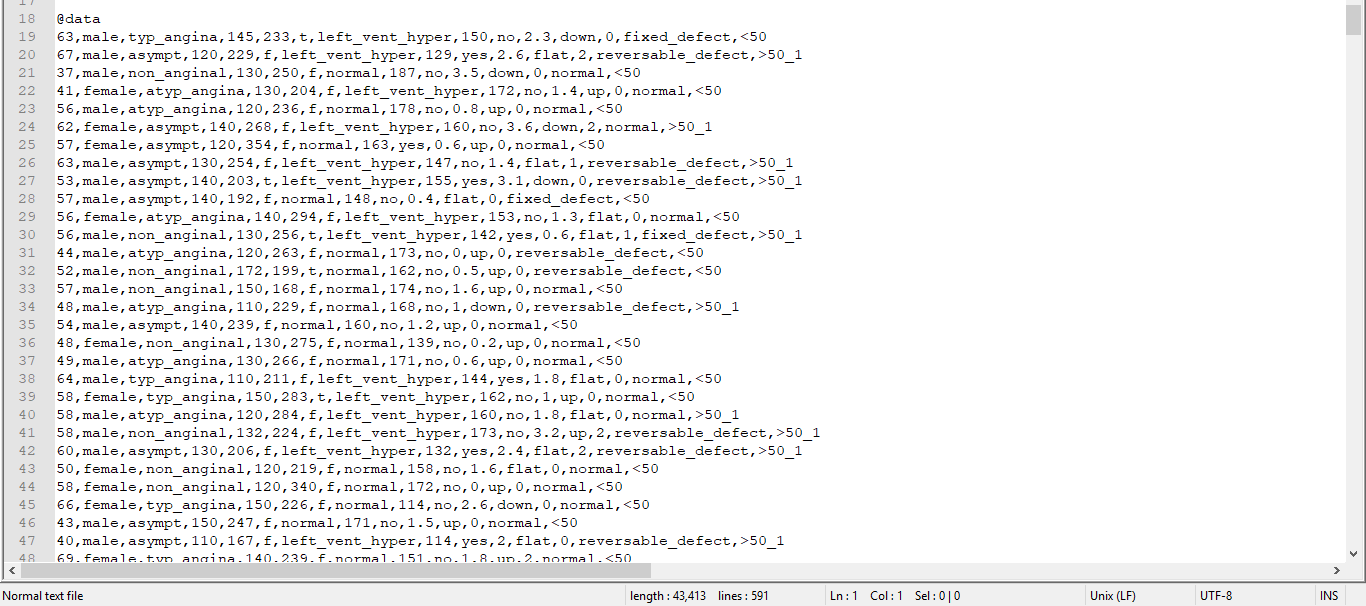
\includegraphics[width=0.98\textwidth]{4/4d.png}
\caption{Sau khi làm sạch.}
\end{figure}
\end{itemize}

%55555555555555555555555555555555555555555555555555555555555
\subsection{Chuyển đổi dữ liệu - Transformation}
\subsubsection{Xây dựng thuộc tính – \textit{Attribute construction}}
Weka hỗ trợ 4 bộ lọc để thêm một thuộc tính mới vào dataset, ta sẽ lần lượt tìm hiểu từng bộ lọc.
\begin{itemize}
	\item \code{attribute.Add}
	\begin{figure}[H]
\centering
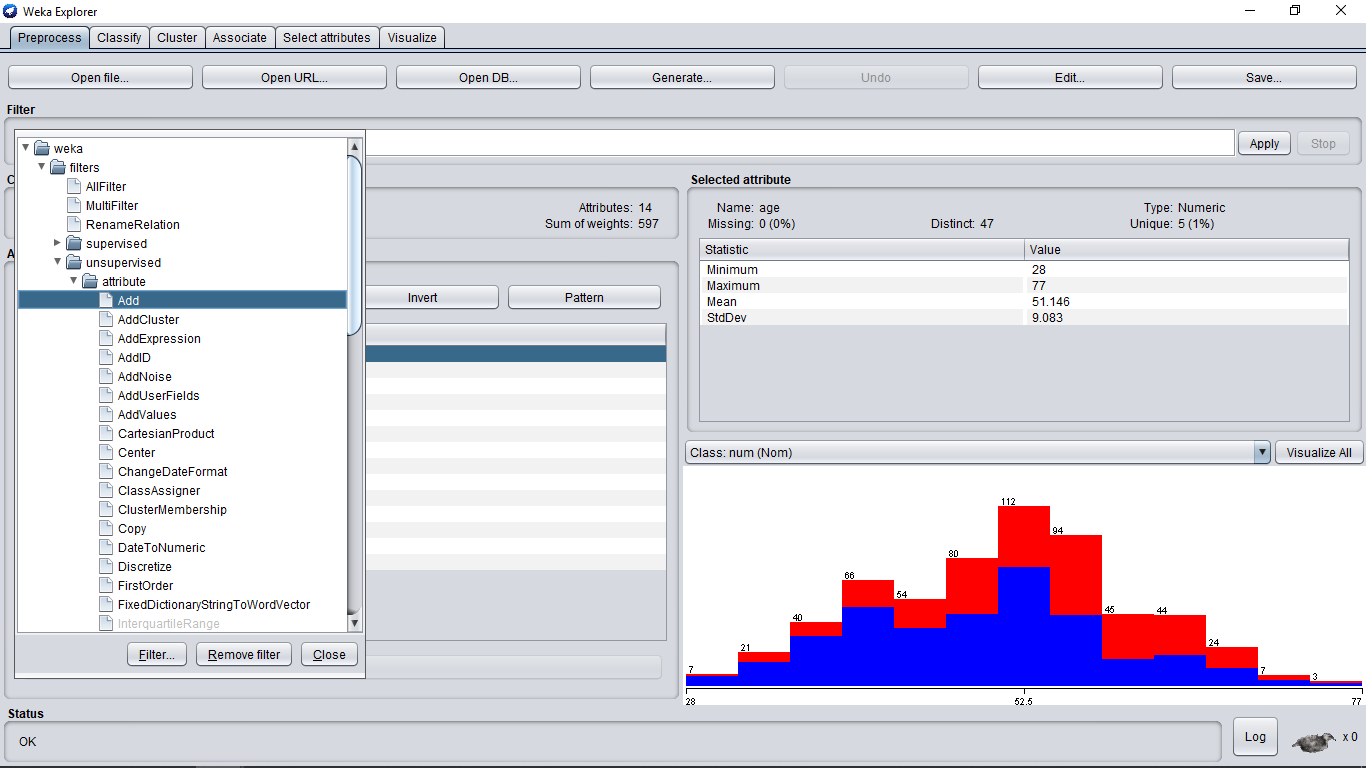
\includegraphics[width=0.98\textwidth]{5/a1.png}
\caption{Ở thanh \textit{Filter}, chọn \textit{$Choose \rightarrow weka \rightarrow filters \rightarrow unsupervised \rightarrow attribute \rightarrow Add$}}
\end{figure}

\begin{figure}[H]
\centering
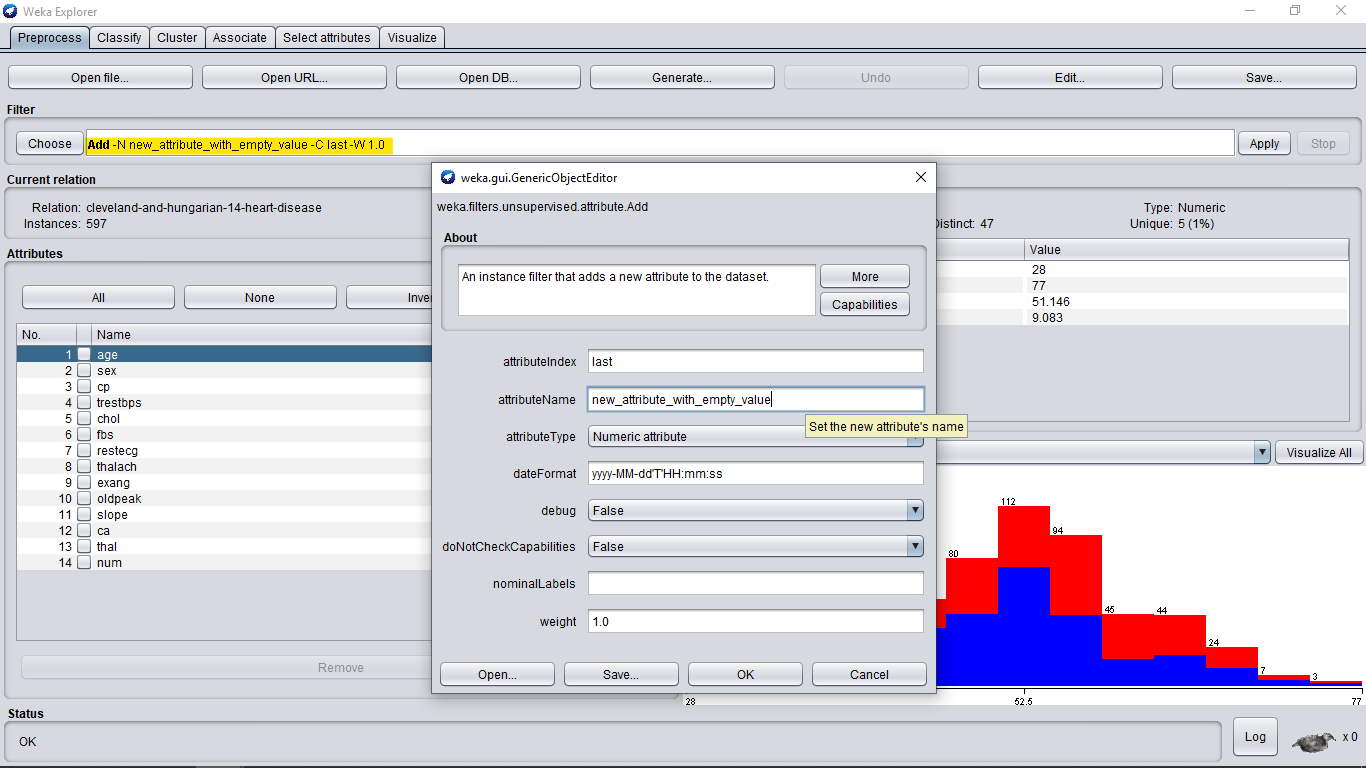
\includegraphics[width=0.98\textwidth]{5/a2.png}
\caption{Nháy vào thanh màu vàng và điền các thông số vào. Thuộc tính mới sẽ có dạng \textit{missing value}.}
\end{figure}

\begin{figure}[H]
\centering
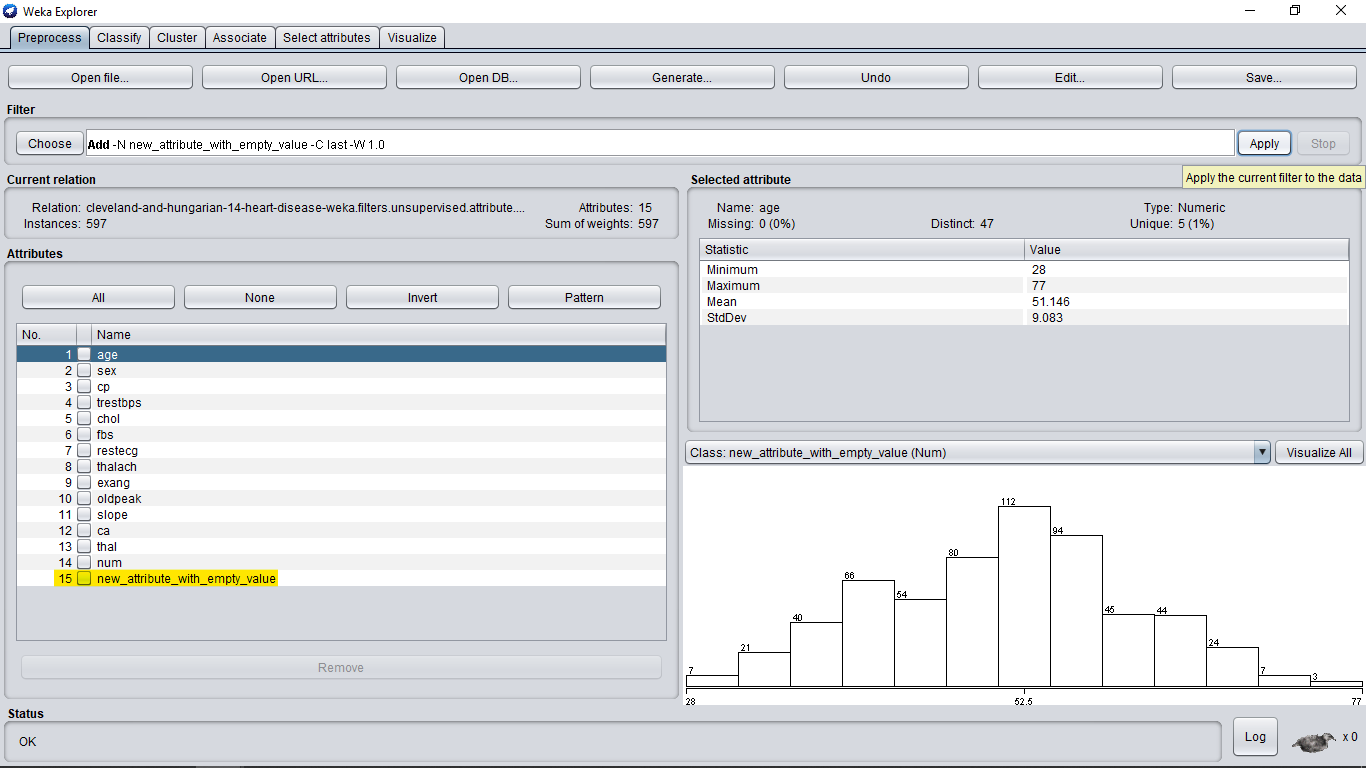
\includegraphics[width=0.98\textwidth]{5/a3.png}
\caption{Nhấn \textit{Apply} để áp dụng bộ lọc, thuộc tính mới sẽ được thêm vào sau đó.}
\end{figure}

\item \code{attribute.AddCluster}\\
Ta thao tác tương tự như \code{attribute.Add}, bộ lọc này sẽ thêm vào một thuộc tính \textit{nomial} thể hiện kết quả phân cụm cho các mẫu khi áp dụng một thuật toán phân cụm nào đó.
\begin{figure}[H]
\centering
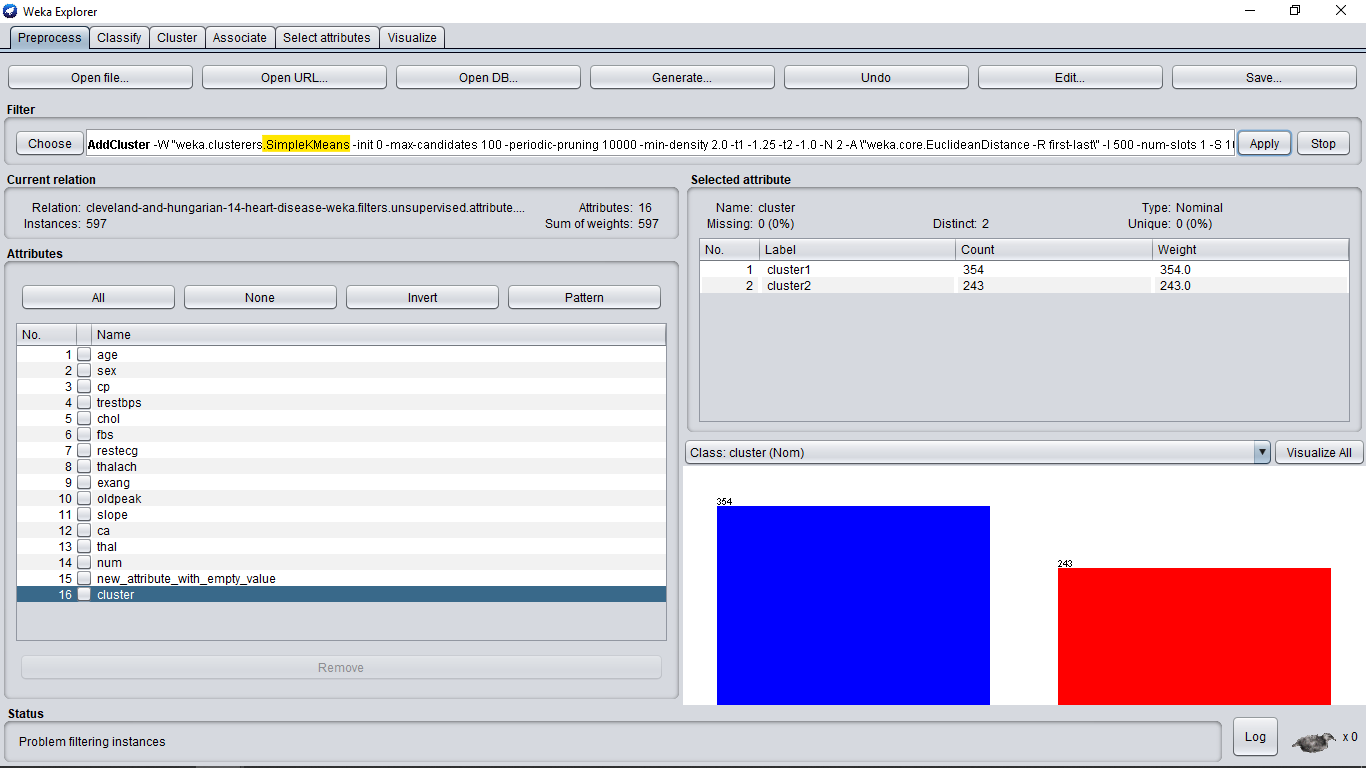
\includegraphics[width=0.98\textwidth]{5/a4.png}
\caption{Thuộc tính \textit{cluster} được thêm vào với thuật toán \textit{SimpleKMeans}.}
\end{figure}

\item \code{attribute.AddExpression}\\
Bộ lọc này sẽ thêm vào một thuộc tính mới bằng cách áp dụng một phép toán nào đó trên những thuộc tính sẵn có.

\begin{figure}[H]
\centering
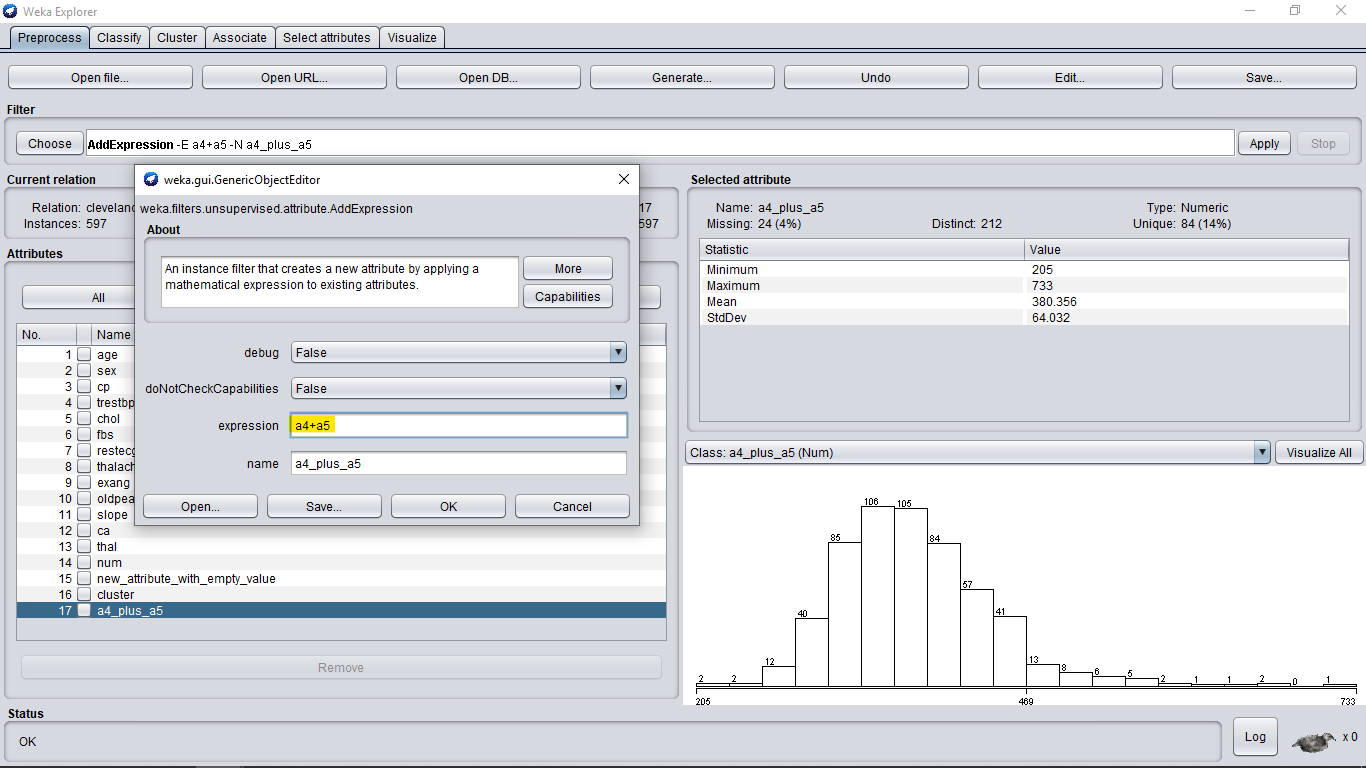
\includegraphics[width=0.98\textwidth]{5/a5.png}
\caption{Thêm một thuộc tính là tổng của hai thuộc tính sẵn có, tên các biến có dạng \code{a+<số thứ tự của thuộc tính>}. Như ví dụ trên là \code{a4+a5}.}
\end{figure}	

\item \code{attribute.AddID}\\Thêm thuộc tính ID vào dataset.
\end{itemize}

\subsubsection{Chuẩn hóa – \textit{Normalize}}
Hai bộ lọc \code{attribute.Normalize} và \code{attribute.Standardize} cho phép chuẩn hóa Min-max và chuẩn hóa Z-score.

\begin{itemize}
	\item \textbf{Chuẩn hóa Min-max}
	\begin{figure}[H]
\centering
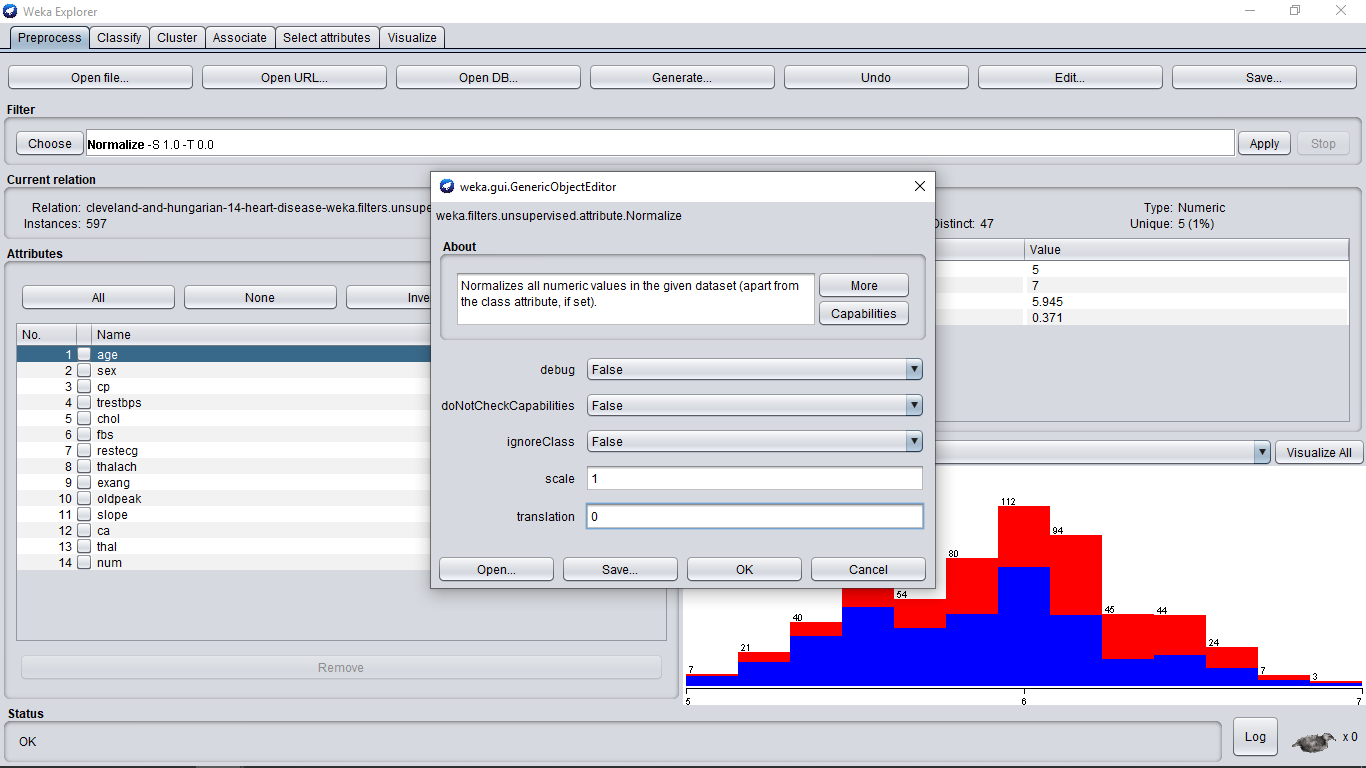
\includegraphics[width=0.98\textwidth]{5/b1.png}
\caption{Ở thanh \textit{Filter}, chọn \textit{$Choose \rightarrow weka \rightarrow filters \rightarrow unsupervised \rightarrow attribute \rightarrow Normalize$}. Trong đó min là \textit{translation}, còn max là \textit{translation + scale}. Ví dụ, với $min=0$, $max=1$, ta điền như trên hình.}
\end{figure}

\begin{figure}[H]
\centering
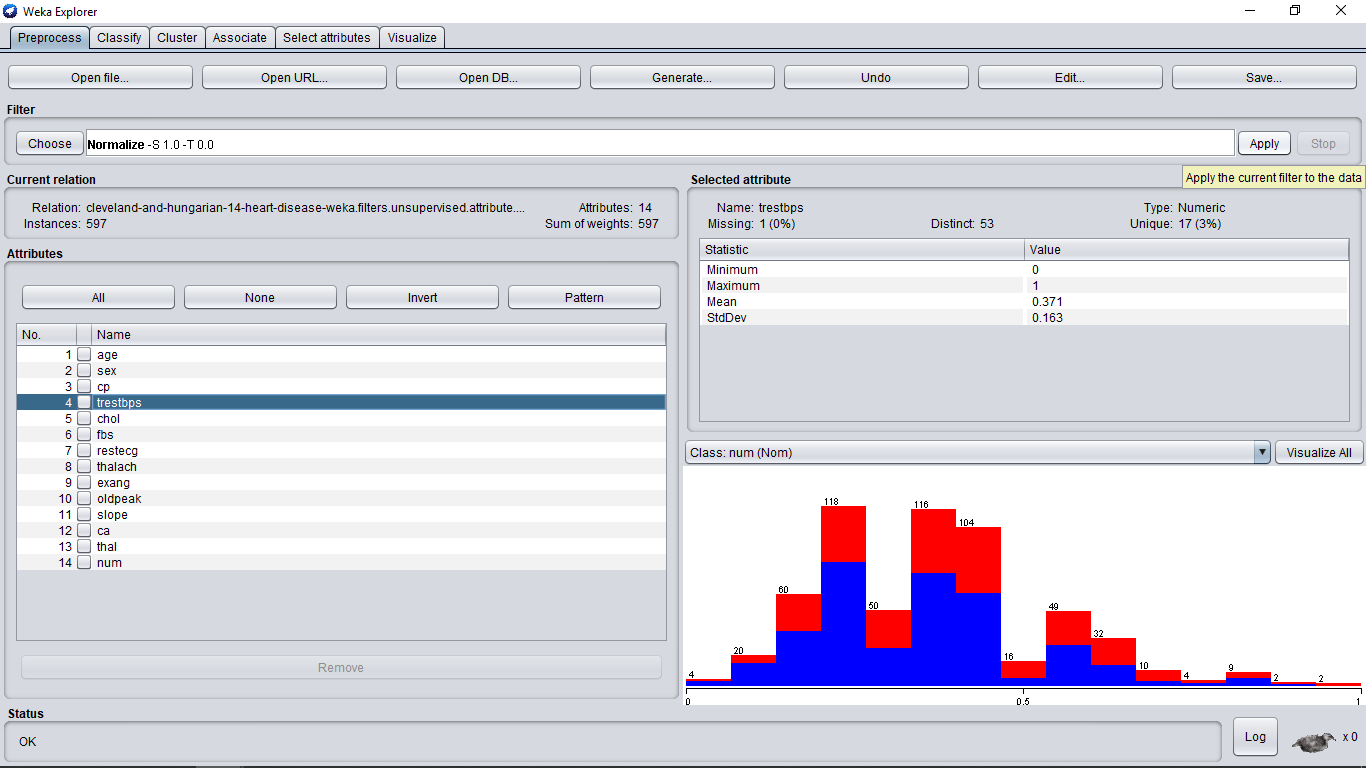
\includegraphics[width=0.98\textwidth]{5/b2.png}
\caption{Nháy \textit{Apply} để chuẩn hóa.}
\end{figure}

\item \textbf{Chuẩn hóa Z-score}
\begin{figure}[H]
\centering
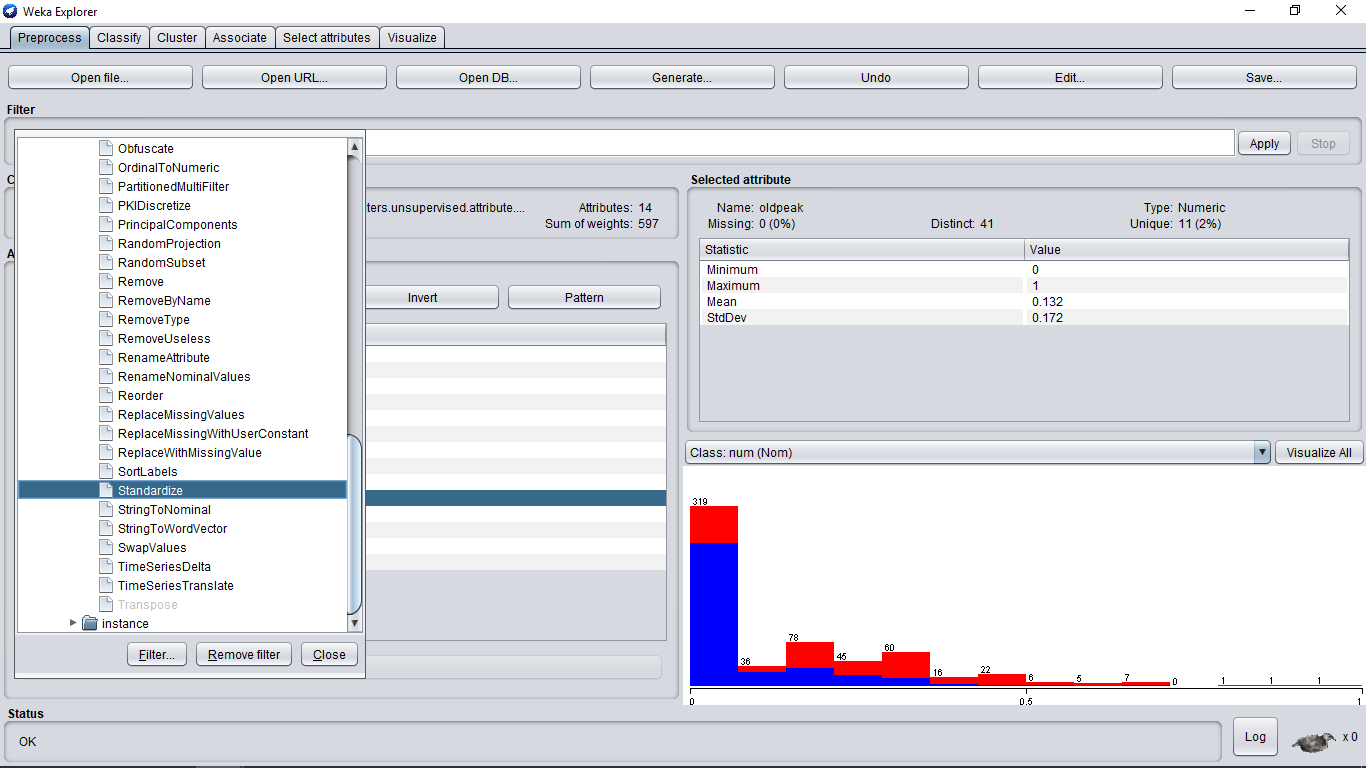
\includegraphics[width=0.98\textwidth]{5/b3.png}
\caption{Ở thanh \textit{Filter}, chọn \textit{$Choose \rightarrow weka \rightarrow filters \rightarrow unsupervised \rightarrow attribute \rightarrow Standardize$}.}
\end{figure}

\begin{figure}[H]
\centering
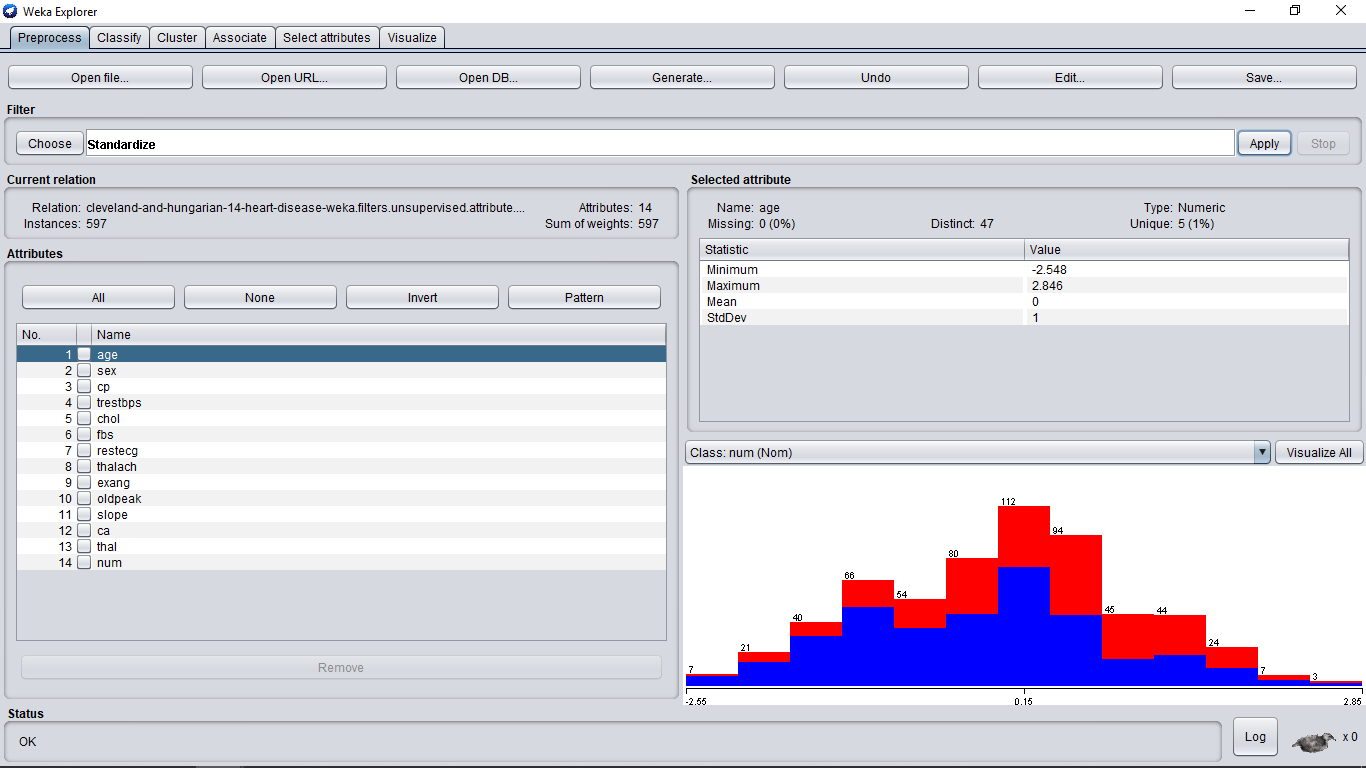
\includegraphics[width=0.98\textwidth]{5/b4.png}
\caption{Nháy \textit{Apply} để chuẩn hóa.}
\end{figure}

\end{itemize}

\subsubsection{Chọn phương pháp chuẩn hóa}
Chọn Z-score vì sẽ thuận lợi trong trường hợp phân phối có Gaussian, đồng thời không từ chối dữ liệu mới nạp vào nằm ngoài min-max như trong chuẩn hóa Min-max.
\begin{figure}[H]
\centering
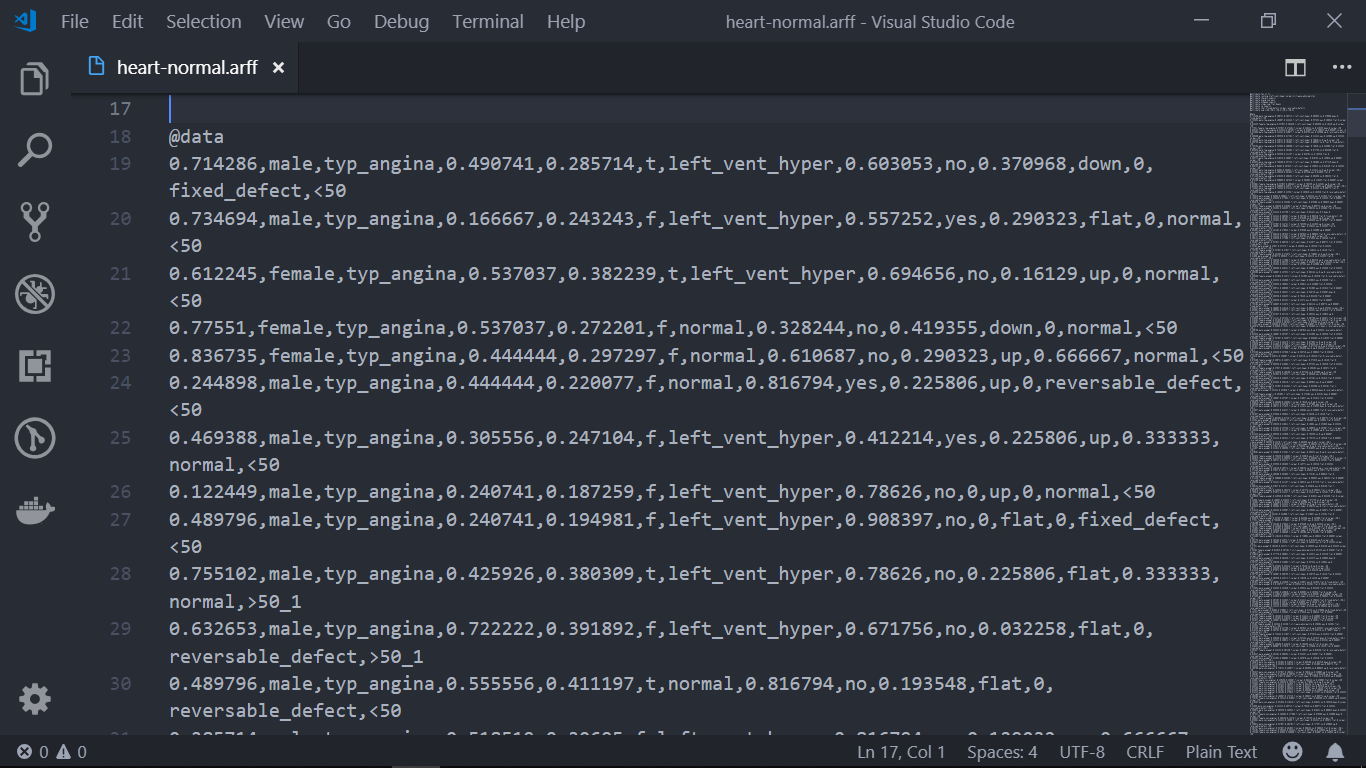
\includegraphics[width=0.98\textwidth]{5/f.png}
\caption{Sau khi chuẩn hóa Z-score.}
\end{figure}

%6666666666666666666666666666666666666666666666666666666666666666
\subsection{Rút gọn dữ liệu - Reduction}
\subsubsection{Lấy mẫu dữ liệu với các bộ lọc Weka}
\begin{itemize}
	\item B1: Ở mục Filter chọn nút Choose $\rightarrow$ supervised (hoặc unsupervised) $\rightarrow$ instance $\rightarrow$ Resample.
	\begin{figure}[H]
\centering
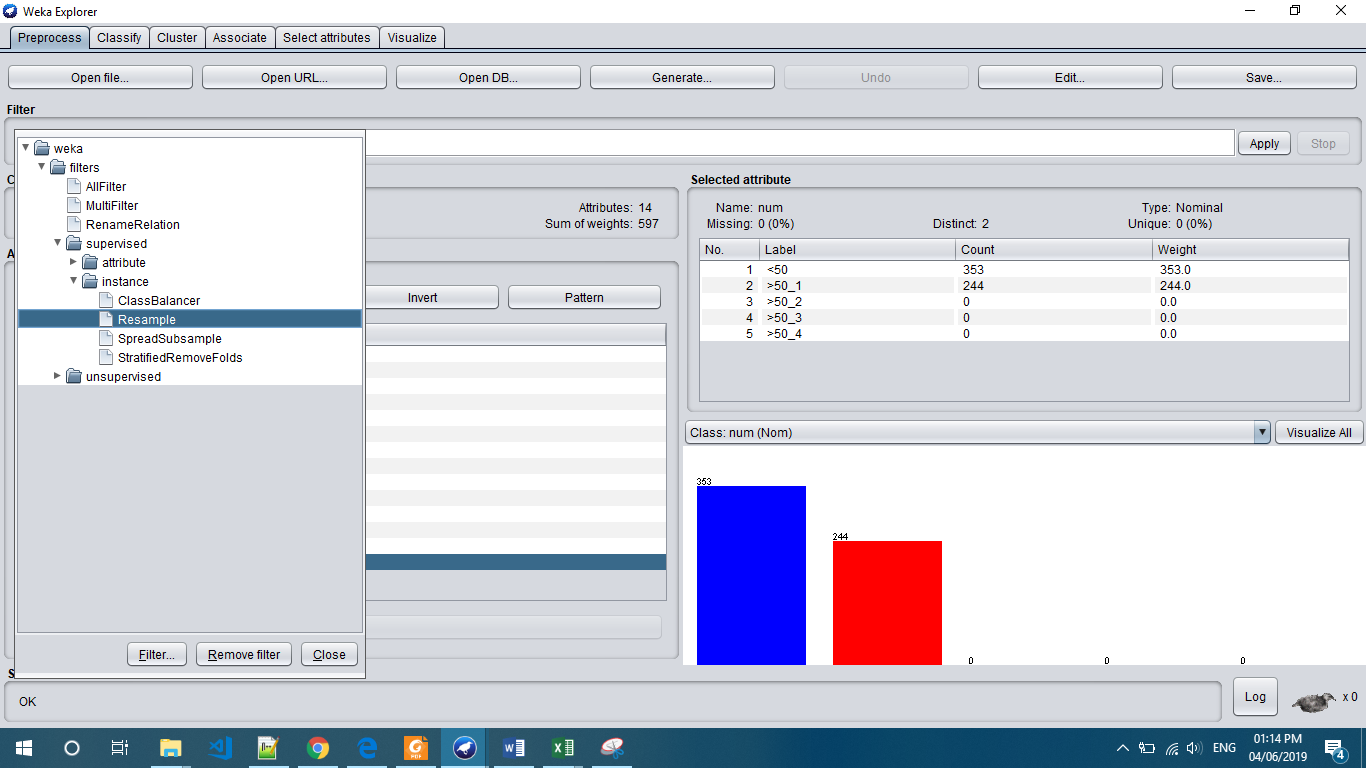
\includegraphics[width=0.98\textwidth]{6/1.png}
%\caption{Sau khi chuẩn hóa Z-score.}
\end{figure}
\item B2: Nhấp chọn ô thông số bên cạnh nút Choose để chỉnh sửa các thông số:
\begin{itemize}
\item	randomSeed: đặt mầm (seed) ngẫu nhiên để lấy mẫu
\item	biasToUniformClass (thông số này chỉ có khi chọn mục supervised): giá trị 0 – phân phối của lớp như hiện trạng (như bộ dữ liệu đầu). Giá trị 1 – phân phối lớp của mẫu là phân phối chuẩn (uniform).
\item	noReplacement: True – with replacement (lấy tuple dữ liệu ra và trả lại nó trong bộ dữ liệu D, nghĩa là có thể nó sẽ vẫn có thể được rút ra trong lần lấy tuple sau). False – without replacement (lấy tuple dữ liệu ra (với xác suất rút 1/N) và không trả nó lại trong bộ dữ liệu D, nghĩa là mỗi tuple chỉ xuất hiện 1 lần trong mẫu).
\item	sampleSizePercent: kích thước của mẫu so với bộ dữ liệu gốc bao nhiêu phần trăm.
\item	invertSelection: lấy mẫu với các bộ ngược lại (inverse) so với mẫu lấy được (chỉ áp dụng với mẫu không có lặp – without replacement).

\end{itemize}
\begin{figure}[H]
\centering
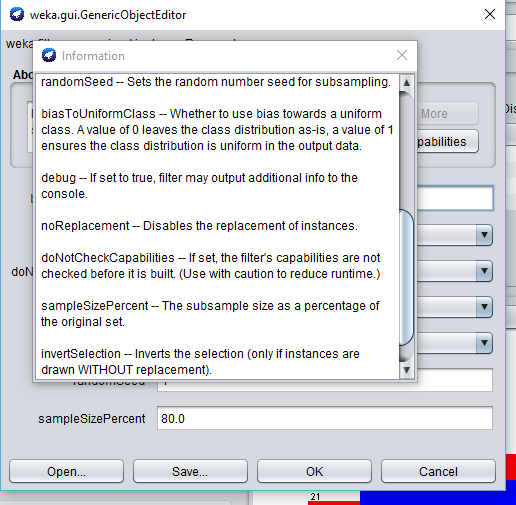
\includegraphics[width=0.98\textwidth]{6/2.png}
%\caption{Sau khi chuẩn hóa Z-score.}
\end{figure}
\item B3: Sau khi chọn các thông số theo nhu cầu, nhấn nút Apply để lấy mẫu (sampling).

\begin{figure}[H]
\centering
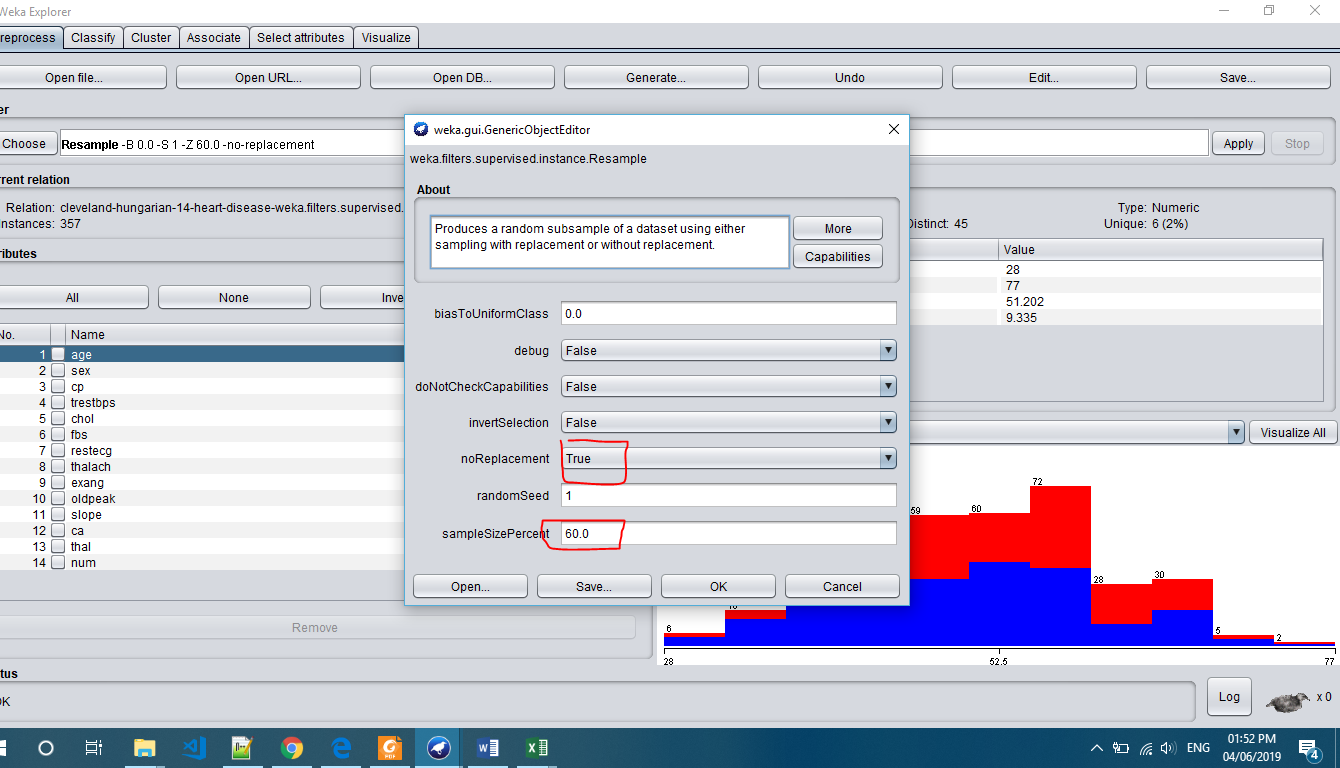
\includegraphics[width=0.98\textwidth]{6/3.png}
\caption{Ví dụ: ở đây nhóm lấy mẫu vói các thông số: noReplacement = True, sampleSize = 60.}
\end{figure}
\begin{figure}[H]
\centering
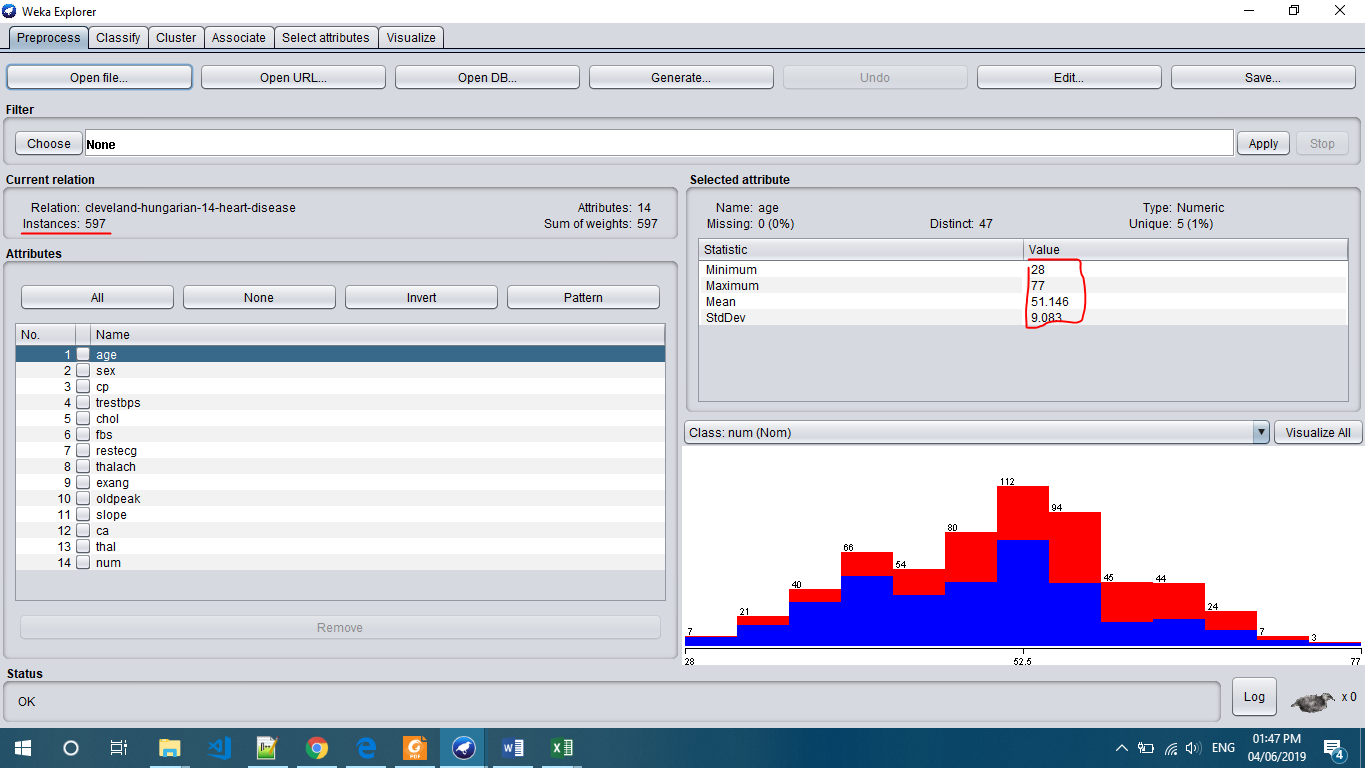
\includegraphics[width=0.98\textwidth]{6/4.png}
\caption{Ảnh bộ dữ liệu gốc.}
\end{figure}
\begin{figure}[H]
\centering
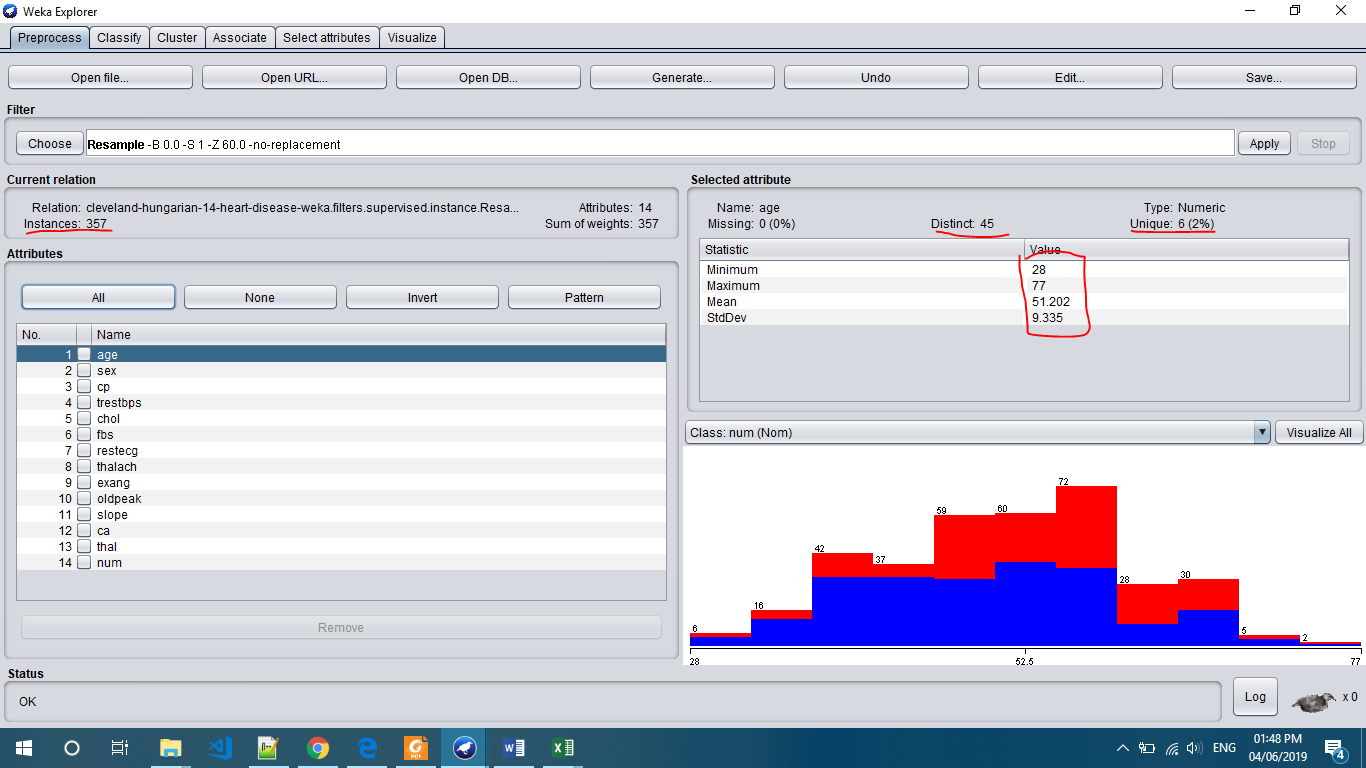
\includegraphics[width=0.98\textwidth]{6/5.png}
\caption{Mẫu lấy được với các thông số như trên.}
\end{figure}
\end{itemize}

\subsubsection{Khả năng thực hiện của Weka}
Trong Weka, ta có thể thực hiện 2 phương pháp chính: Simple Random Sample Without Replace (SRSWOR) và Simple Random Sample With Replacement (SRSWR) bằng cách đặt thông số option noReplacement là True (không lặp) hoặc False (có lặp).

%\subsection{Phát hiện biên cạnh sử dụng Sobel}
%Toán tử Sobel:
%\[
%	Wx=\begin{bmatrix} 
%	0.25 & 0 & -0.25 \\
%	0.5 & 0 & -0.5 \\
%	0.25 & 0 & -0.25
%	\end{bmatrix}
%	,\hspace*{30pt}
%	Wy=\begin{bmatrix} 
%	-0.25 & -0.5 & -0.25 \\
%	0 & 0 & 0 \\
%	0.25 & 0.5 & 0.25
%	\end{bmatrix}
%\]
%\begin{itemize}
%	\item[--]$Gx$ là ma trận ảnh đạo hàm theo $x$ (Gradient x) được tính bằng cách nhân tích chập với ma trận $Wx$.
%	\item[--]$Gy$ là ma trận ảnh đạo hàm theo $y$ (Gradient y) được tính bằng cách nhân tích chập với ma trận $Wy$.
%	\item[--]$G$ là ma trận Gradient áp dụng Sobel được tính bằng $\lvert {Gx} + {Gy}\rvert$ hoặc $\sqrt{(Gx)^2 + (Gy)^2}$
%\end{itemize}
%
%\subsection{Phát hiện biên cạnh sử dụng Prewitt}
%Toán tử Prewitt:
%\[
%	Wx=\begin{bmatrix} 
%	\frac{1}{3} & 0 & \frac{-1}{3} \\
%	\frac{1}{3} & 0 & \frac{-1}{3} \\
%	\frac{1}{3} & 0 & \frac{-1}{3}
%	\end{bmatrix}
%	,\hspace*{30pt}
%	Wy=\begin{bmatrix} 
%	\frac{-1}{3} & \frac{-1}{3} & \frac{-1}{3} \\
%	0 & 0 & 0 \\
%	\frac{1}{3} & \frac{1}{3} & \frac{1}{3}
%	\end{bmatrix}
%\]
%\begin{itemize}
%	\item[--]$Gx$ là ma trận ảnh đạo hàm theo $x$ (Gradient x) được tính bằng cách nhân tích chập với ma trận $Wx$.
%	\item[--]$Gy$ là ma trận ảnh đạo hàm theo $y$ (Gradient y) được tính bằng cách nhân tích chập với ma trận $Wy$.
%	\item[--]$G$ là ma trận Gradient áp dụng Sobel được tính bằng $\lvert {Gx} + {Gy}\rvert$ hoặc $\sqrt{(Gx)^2 + (Gy)^2}$
%\end{itemize}
%
%\subsection{Phát hiện biên cạnh sử dụng Laplace}
%Ma trận WLap:
%\begin{center}
%$W=\begin{bmatrix} 
%	0 & 1 & 0 \\
%	1 & -4 & 1 \\
%	0 & 1 & 0
%	\end{bmatrix}$
%	\textit{hoặc}\hspace*{30pt}
%	$W=\begin{bmatrix} 
%	1 & 1 & 1 \\
%	1 & -8 & 1 \\
%	1 & 1 & 1
%	\end{bmatrix}$
%\end{center}
%
%\subsection{Phát hiện biên cạnh sử dụng Canny}
%\begin{itemize}
%	\item[--] Làm trơn ảnh
%	\item[--] Tính đạo hàm ảnh
%	\item[--] Tìm hướng biên cạnh
%	\item[--] Non-maxmimum suppression
%	\item[--] Hysteresis
%\end{itemize}

\newpage